\documentclass[11pt]{article}
\usepackage[margin=1in]{geometry}
\usepackage{graphicx}
\usepackage{booktabs}
\usepackage{tabularx}
\usepackage{longtable}
\usepackage{array}
\usepackage{amsmath}
\usepackage{hyperref}
\usepackage{float}
\usepackage{pdflscape}

\graphicspath{{handbook_assets/}}
\hypersetup{
    colorlinks=true,
    linkcolor=blue,
    urlcolor=blue,
    pdftitle={ADCS Simulink Model Reading Guide},
    pdfauthor={OpenAI Codex}
}

\newcolumntype{Y}{>{\raggedright\arraybackslash}X}
\setlength{\parskip}{0.55em}
\setlength{\parindent}{0pt}

\title{\textbf{ADCS Simulink Model Reading Guide}\\
\large A technical handbook for understanding the \texttt{adcs-sim} model}
\author{Prepared from the repository source of truth}
\date{April 23, 2026}

\begin{document}
\maketitle

\begin{abstract}
This handbook explains how to read the \texttt{adcs-sim} MATLAB/Simulink model as it exists in the repository today. It is written for a beginner who can open the model and recognize blocks and connectors, but cannot yet tell what each signal means, how the subsystems fit together, or where to look in the source tree when the diagram alone is not enough. The guide covers the architecture, inputs, outputs, GUI controls, signal flow, subsystem responsibilities, key equations, and current modeling limitations. It also distinguishes clearly between the simulator architecture that the project is designed to support and the compile-safe fallback behavior that several blocks currently use in the validated branch.
\end{abstract}

\section*{Executive Summary}
\addcontentsline{toc}{section}{Executive Summary}

The most important fact to understand before reading this model is that the generated \texttt{adcs\_sim.slx} file is \textbf{not} the real source of truth. The source of truth is the MATLAB code that builds the model:

\begin{verbatim}
build_adcs_model.m  ->  builders/build_*.m  ->  adcs_sim.slx
\end{verbatim}

For a beginner, that one fact removes most of the confusion. If a connector is visually hard to follow in Simulink, the definitive answer is usually in one of three places:

\begin{enumerate}
\item \texttt{build\_adcs\_model.m}, where top-level subsystems and cross-subsystem lines are created.
\item \texttt{reference.md}, which lists port orders and signal names in plain language.
\item The relevant builder file in \texttt{builders/}, where the subsystem interface and internal block logic are declared.
\end{enumerate}

At a high level, the model is organized as a left-to-right closed-loop chain:

\begin{verbatim}
ENVIRONMENT -> SENSORS -> CONTROL -> ACTUATORS -> DYNAMICS -> workspace logs
                    ^                                      |
                    +------------- feedback --------------+
\end{verbatim}

That loop is the conceptual backbone of the project:

\begin{itemize}
\item \textbf{ENVIRONMENT} provides truth-side orbital and environmental quantities such as Sun direction, Moon direction, magnetic field, position, velocity, and eclipse state.
\item \textbf{SENSORS} converts truth-side states into measurements such as attitude, angular rate, body-frame Sun vector, body-frame magnetic field, and GNSS-like position and velocity.
\item \textbf{CONTROL} consumes measurements and decides what the spacecraft should do.
\item \textbf{ACTUATORS} convert those commands into torques or momentum-change signals.
\item \textbf{DYNAMICS} integrates the rotational state and feeds true attitude and rate back into the sensor models.
\item \textbf{To Workspace} blocks save the main state histories for post-processing and GUI display.
\end{itemize}

The second critical fact is that the current validated branch is \textbf{architecturally comprehensive but behaviorally mixed-fidelity}. The dataflow is real and the rigid-body attitude dynamics path is meaningful, but several blocks presently run compile-safe fallback implementations. In particular:

\begin{itemize}
\item Orbit propagation is currently a fixed finite LEO state fallback.
\item Magnetic field is currently a constant-vector fallback.
\item Eclipse is currently a constant sunlit fallback.
\item Star tracker, IMU, and GNSS are currently passthrough sensor fallbacks.
\item The onboard ephemeris, reference generator, mode manager, control law, reaction wheel assembly, magnetorquer assembly, and CMG are all currently simplified fallback implementations.
\item The main physically active pieces in the validated branch are quaternion kinematics, quaternion normalization, rigid-body rotational dynamics, and gravity-gradient torque.
\end{itemize}

That means this handbook should be read in two layers:

\begin{itemize}
\item \textbf{Layer 1: architecture and interfaces.} These are already worth studying and are stable enough to understand the intended ADCS pipeline.
\item \textbf{Layer 2: present numerical fidelity.} This is only partial in the current branch and must be described honestly.
\end{itemize}

\tableofcontents
\clearpage

\section{What the Model Is}

The repository contains a programmatic MATLAB/Simulink attitude determination and control system simulator for a 3U-class CubeSat mission. The simulator is organized around the canonical ADCS pipeline:

\begin{verbatim}
truth environment -> sensors -> estimation/control -> actuators -> dynamics
\end{verbatim}

The files that matter most when you want to understand the model are shown in Table \ref{tab:source-of-truth-files}.

\begin{table}[H]
\centering
\begin{tabularx}{\textwidth}{@{}lY@{}}
\toprule
\textbf{File} & \textbf{Why it matters} \\
\midrule
\texttt{README.md} & High-level entry point, quick start, and repository map. \\
\texttt{build\_adcs\_model.m} & Creates the top-level model, declares top-level subsystem blocks, and defines cross-subsystem signal routing. \\
\texttt{builders/build\_environment.m} & Defines the ENVIRONMENT subsystem interface and its embedded MATLAB Function logic. \\
\texttt{builders/build\_sensors.m} & Defines the SENSORS subsystem and how truth states are converted into measurements. \\
\texttt{builders/build\_control.m} & Defines the CONTROL subsystem and how measurements map to commands. \\
\texttt{builders/build\_actuators.m} & Defines the ACTUATORS subsystem and its torque-generation interfaces. \\
\texttt{builders/build\_dynamics.m} & Defines the DYNAMICS subsystem, integrators, disturbance terms, and state feedback. \\
\texttt{init\_adcs\_params.m} & Loads base-workspace parameters, ephemeris arrays, spacecraft properties, sensor properties, actuator limits, and simulation settings. \\
\texttt{launch\_adcs\_gui.m} & Defines the current interactive dashboard and therefore the actual user-facing controls. \\
\texttt{simulate\_adcs\_case.m} & Shows the run workflow: initialize parameters, apply overrides, rebuild the model, simulate, summarize. \\
\texttt{summarize\_adcs\_simulation.m} & Defines the derived metrics and the exact meaning of the main logged outputs. \\
\texttt{reference.md} & Plain-language architecture, port map, and parameter quick-reference. \\
\texttt{skills.md} & Domain notes for the intended physics, estimation, and control models. \\
\bottomrule
\end{tabularx}
\caption{Files that function as the real source of truth when reading the model.}
\label{tab:source-of-truth-files}
\end{table}

\subsection{Generated versus authored content}

\texttt{adcs\_sim.slx} is generated output. It is useful for visualization, but it is not the best place to answer questions such as ``what does port 4 mean?'' or ``where does this line come from?'' Those answers live in the builders and in the top-level build script.

\section{How to Read the Model Without Getting Lost}

The beginner-friendly way to read this project is:

\begin{enumerate}
\item Open \texttt{README.md} and \texttt{reference.md} first.
\item Open \texttt{build\_adcs\_model.m} and read the comments above the top-level routing.
\item Open the top-level Simulink model and identify the five major subsystems from left to right.
\item For any connector that is unclear, look up the source and destination port order in \texttt{build\_adcs\_model.m} or \texttt{reference.md}.
\item If a block inside a subsystem is unclear, open the matching \texttt{builders/build\_*.m} file and read the embedded MATLAB Function code generator for that block.
\item Use \texttt{init\_adcs\_params.m} to understand where each constant, initial condition, and limit comes from.
\item Use \texttt{summarize\_adcs\_simulation.m} to understand what the logged outputs are later turned into.
\end{enumerate}

In other words: use the diagram to orient yourself, and use the MATLAB source to disambiguate the diagram.

\subsection{How connectors work in this project}

Most of the confusion in a generated Simulink model comes from the fact that lines are created by port number, not by prose. This project is unusually readable once you know that the builder comments document the port contract explicitly.

Example:

\begin{verbatim}
ENVIRONMENT output port mapping:
  1 = Sun_vec_ECI   2 = Moon_vec_ECI   3 = B_ECI
  4 = pos_ECI       5 = vel_ECI        6 = eclipse_flag
\end{verbatim}

Therefore this line in the source:

\begin{verbatim}
add_line(mdl, 'ENVIRONMENT/1', 'SENSORS/3', ...)
\end{verbatim}

means:

\begin{verbatim}
Sun_vec_ECI  ->  Sun_ECI
\end{verbatim}

Once you adopt that reading style, the model becomes much easier to follow.

\section{End-to-End Simulation Workflow}

The run pipeline from parameters to outputs is shown below:

\begin{verbatim}
init_adcs_params
    |
    +-- loads constants, initial conditions, ephemeris arrays, orbit data,
        sensor specs, actuator limits, and simulation settings into the base workspace
    |
build_adcs_model
    |
    +-- creates the top-level Simulink model and subsystem internals
    |
sim('adcs_sim')
    |
    +-- propagates the model and logs q_log, omega_log, h_W_log
    |
summarize_adcs_simulation
    |
    +-- derives excursion, norm error, peak/rms rates, kinetic energy,
        wheel utilization, and total angular momentum metrics
    |
launch_adcs_gui
    |
    +-- displays plots, metrics, and the effective parameter set
\end{verbatim}

\subsection{What the GUI actually does}

The GUI is not an alternate simulation engine. It is a front-end around the same standard sequence:

\begin{verbatim}
init_adcs_params -> apply selected overrides -> build_adcs_model -> sim -> summarize
\end{verbatim}

The GUI therefore changes the run by changing selected workspace values before the model is rebuilt and simulated.

\section{Top-Level Architecture and Data Flow}

Figure \ref{fig:top-level-model} shows the generated top-level Simulink diagram. Read it left to right first, then notice the feedback lines from DYNAMICS back to SENSORS and CONTROL.

\begin{figure}[H]
\centering
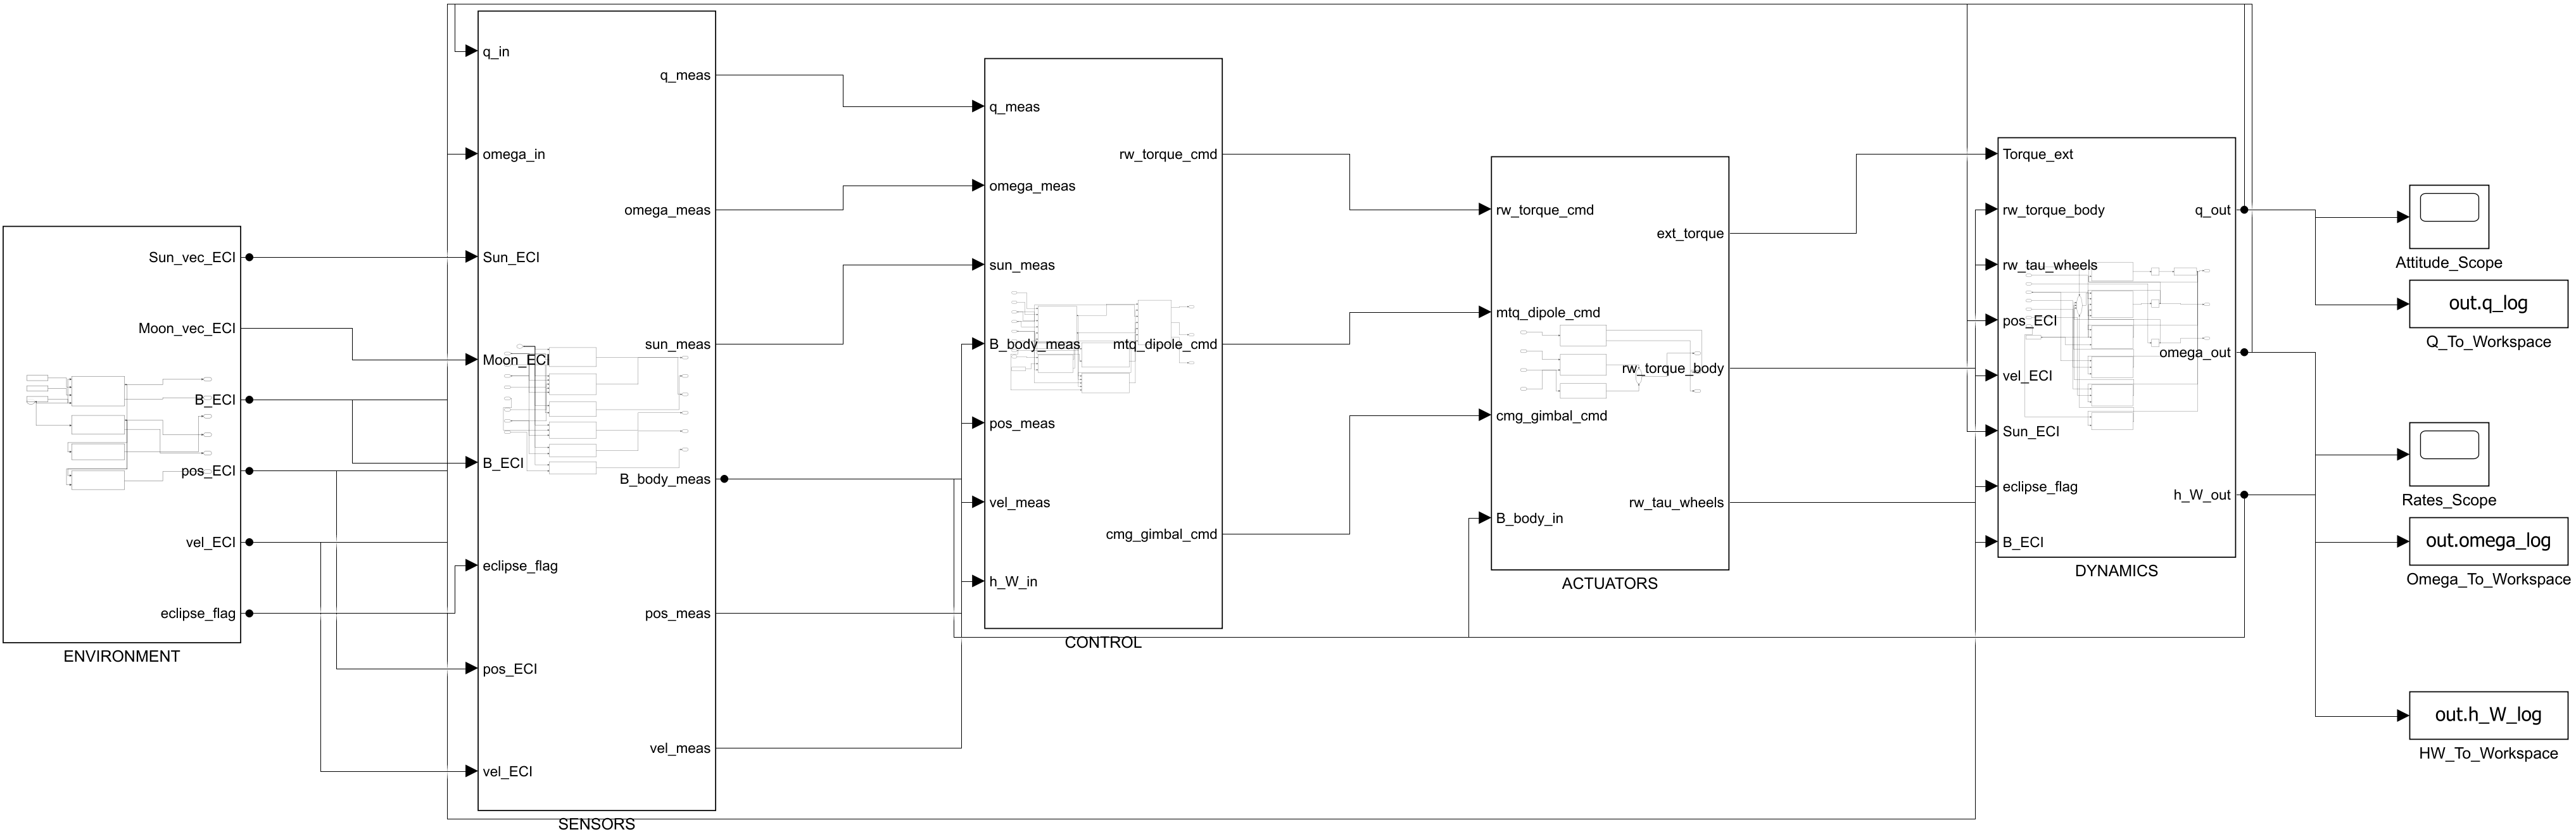
\includegraphics[width=\textwidth]{top_level_model.png}
\caption{Top-level generated Simulink model. The structure is left-to-right, but it closes the loop through attitude and rate feedback from DYNAMICS back into SENSORS, and wheel-momentum feedback from DYNAMICS into CONTROL.}
\label{fig:top-level-model}
\end{figure}

\subsection{Top-level signal flow}

Table \ref{tab:top-level-signal-flow} summarizes the main cross-subsystem lines.

\begin{table}[H]
\centering
\begin{tabularx}{\textwidth}{@{}l l Y@{}}
\toprule
\textbf{From} & \textbf{To} & \textbf{Signals} \\
\midrule
ENVIRONMENT & SENSORS & \texttt{Sun\_vec\_ECI}, \texttt{Moon\_vec\_ECI}, \texttt{B\_ECI}, \texttt{pos\_ECI}, \texttt{vel\_ECI}, \texttt{eclipse\_flag} \\
SENSORS & CONTROL & \texttt{q\_meas}, \texttt{omega\_meas}, \texttt{sun\_meas}, \texttt{B\_body\_meas}, \texttt{pos\_meas}, \texttt{vel\_meas} \\
DYNAMICS & CONTROL & \texttt{h\_W\_out} \\
CONTROL & ACTUATORS & \texttt{rw\_torque\_cmd}, \texttt{mtq\_dipole\_cmd}, \texttt{cmg\_gimbal\_cmd} \\
SENSORS & ACTUATORS & \texttt{B\_body\_meas} for magnetorquer torque computation \\
ACTUATORS & DYNAMICS & \texttt{ext\_torque}, \texttt{rw\_torque\_body}, \texttt{rw\_tau\_wheels} \\
DYNAMICS & SENSORS & \texttt{q\_out}, \texttt{omega\_out} as truth feedback \\
DYNAMICS & Workspace & \texttt{q\_log}, \texttt{omega\_log}, \texttt{h\_W\_log} through To Workspace blocks \\
\bottomrule
\end{tabularx}
\caption{Top-level dataflow across the major subsystems.}
\label{tab:top-level-signal-flow}
\end{table}

\subsection{What this architecture means physically}

The simulator is trying to express the following idea:

\begin{enumerate}
\item The spacecraft exists in an orbital environment with sunlight, Earth magnetic field, position, velocity, and eclipse state.
\item Sensors do not see the ``truth'' perfectly; they produce measurements derived from the truth state.
\item Control logic interprets those measurements and decides what torques or actuator commands to apply.
\item Actuators turn those commands into body torques or internal momentum changes.
\item Dynamics integrates the rotational equations of motion and updates the true attitude, body rate, and reaction-wheel momentum state.
\item Those updated truths become the next sensor inputs, and the loop continues.
\end{enumerate}

\section{Inputs to the Model}

There are three distinct kinds of inputs:

\begin{enumerate}
\item \textbf{Base-workspace parameters} from \texttt{init\_adcs\_params.m}.
\item \textbf{Ephemeris data} from \texttt{ephemeris\_2026\_weekly.csv}.
\item \textbf{GUI override fields} exposed by \texttt{launch\_adcs\_gui.m}.
\end{enumerate}

\subsection{Base-workspace parameter categories}

The model takes many workspace parameters, but they are easier to understand if grouped by role rather than by variable name. Table \ref{tab:input-categories} shows the categories that matter most to a new reader.

\begin{longtable}{@{}p{0.26\textwidth}p{0.68\textwidth}@{}}
\toprule
\textbf{Category} & \textbf{What it includes} \\
\midrule
\endhead
Spacecraft properties & Mass, inertia tensor, 3U geometry, face normals, face areas, and center-of-pressure offsets used by disturbance models. \\
Initial attitude state & Initial quaternion \texttt{q0}. \\
Initial rotational state & Initial body rate \texttt{omega0} and initial reaction-wheel momentum \texttt{h\_W0}. \\
Simulation settings & Fixed-step size \texttt{dt} and run length \texttt{t\_end}. \\
Ephemeris truth arrays & Time grid, Sun vectors, and Moon vectors loaded from CSV. \\
Orbit parameters & Earth constants, altitude, inclination, eccentricity, RAAN, argument of perigee, true anomaly, orbital period, and mean motion. \\
Sensor parameters & FSS noise and field of view, star-tracker exclusion angles and rates, IMU error parameters, magnetometer bias and noise, GNSS noise and sample rates. \\
Actuator parameters & Reaction wheel torque, momentum, speed, inertia, geometry; magnetorquer max dipole; CMG torque and momentum limits. \\
Control parameters & PD gains, B-dot gain, dump gain, unload threshold, and mode thresholds. \\
Environmental constants & Solar flux, speed of light, Earth magnetic-dipole anchor, atmospheric density anchor, drag coefficient, SRP coefficient, residual dipole. \\
Estimator tuning & Noise proxies used by the intended TRIAD/MEKF path. \\
\bottomrule
\caption{High-level categories of workspace inputs loaded before simulation.}
\label{tab:input-categories}
\end{longtable}

\subsection{CSV ephemeris input}

The file \texttt{ephemeris\_2026\_weekly.csv} provides timestamped Sun and Moon direction vectors. In the current validated branch, the \texttt{Ephemeris\_Truth} block interpolates these arrays to produce the truth-side \texttt{Sun\_vec\_ECI} and \texttt{Moon\_vec\_ECI} signals. This means that even though several other environment blocks are presently simplified, the Sun and Moon direction path is still grounded in preloaded ephemeris data rather than a hard-coded constant.

\subsection{GUI controls}

Figure \ref{fig:gui-inputs} shows the current dashboard as implemented in \texttt{launch\_adcs\_gui.m}.

\begin{figure}[H]
\centering
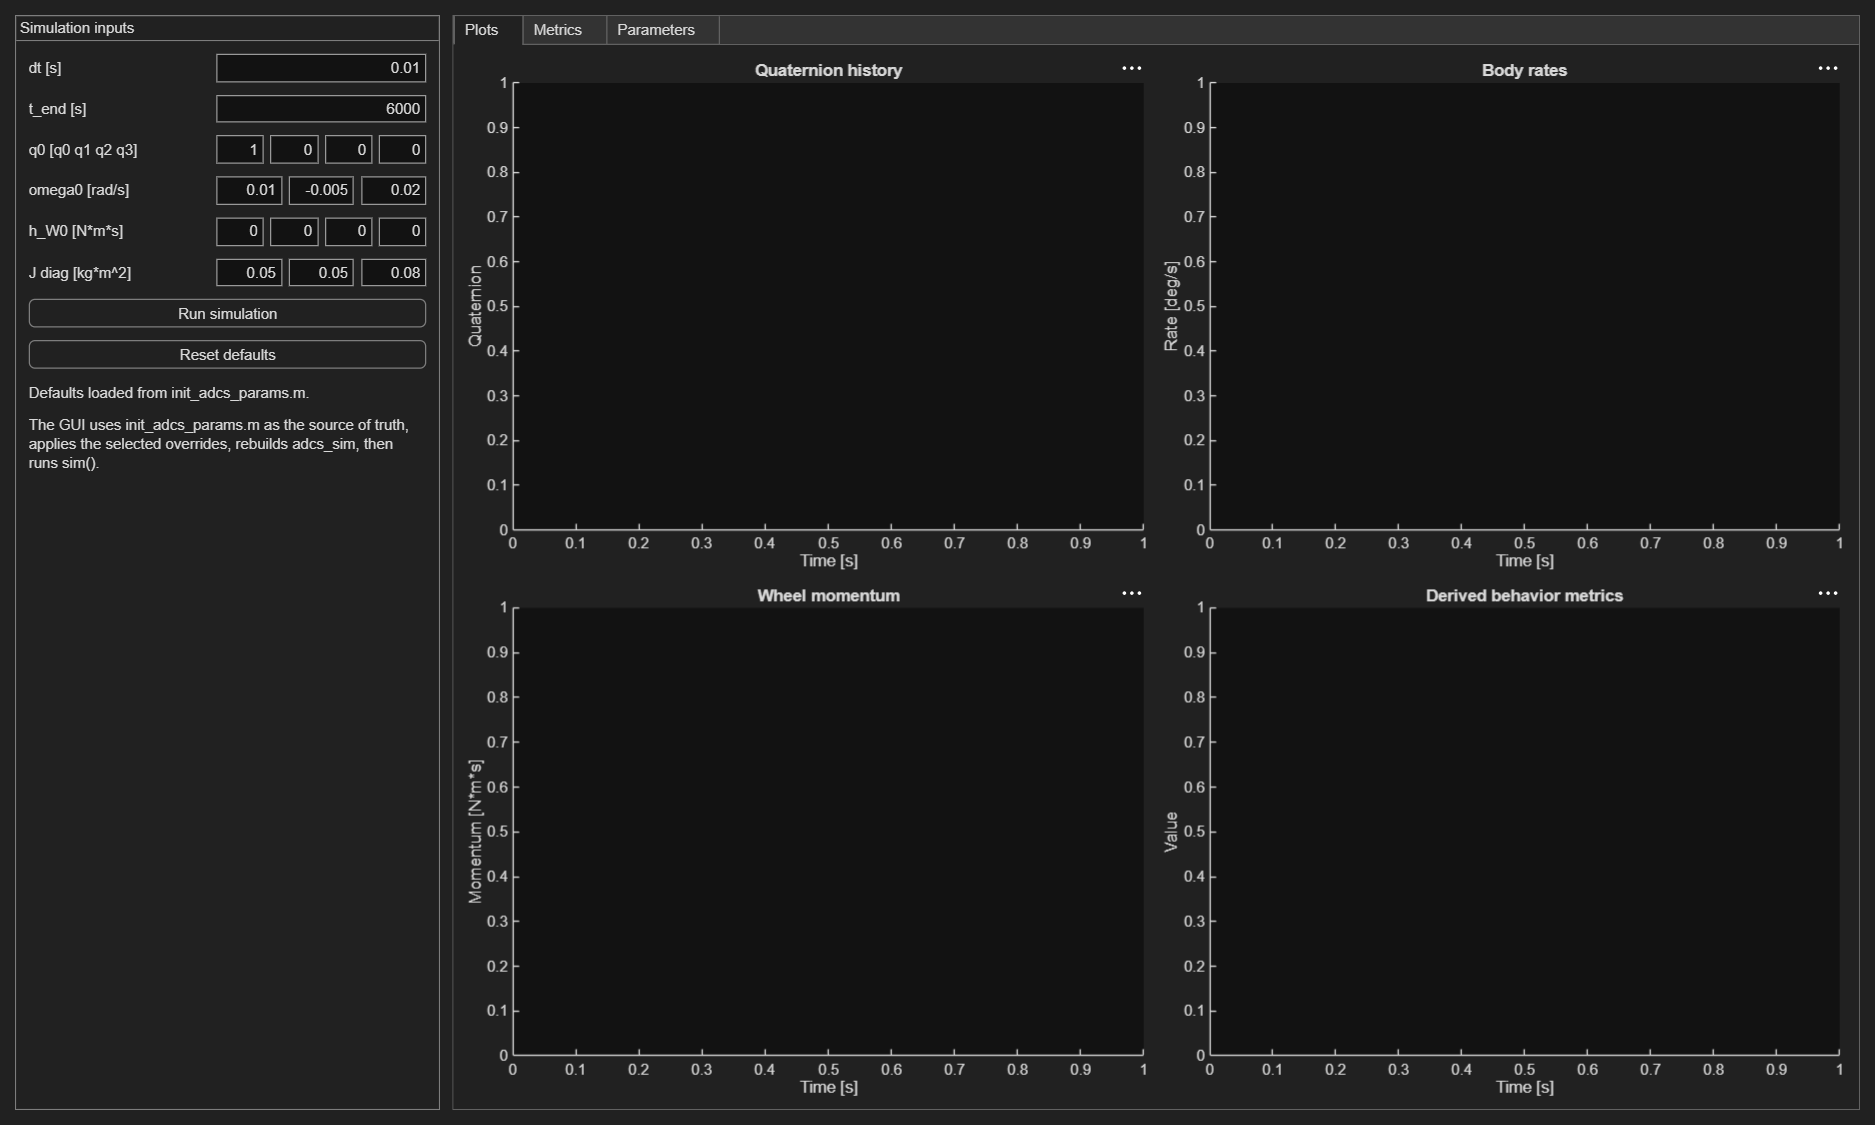
\includegraphics[width=\textwidth]{gui_inputs.png}
\caption{Current GUI before running a simulation. The source-controlled GUI uses numeric edit fields, not sliders.}
\label{fig:gui-inputs}
\end{figure}

\textbf{Important clarification:} the current GUI does \emph{not} contain sliders anywhere in the source-controlled code. It uses numeric input fields instead. For the purpose of understanding the model, these numeric fields are the controls that determine the run.

Table \ref{tab:gui-controls} explains what each control changes and how that affects the spacecraft behavior represented by the model.

\begin{table}[H]
\centering
\begin{tabularx}{\textwidth}{@{}lY Y@{}}
\toprule
\textbf{Control} & \textbf{What it changes in the model} & \textbf{Expected effect on behavior} \\
\midrule
\texttt{dt [s]} & Fixed solver step used by the top-level model. & Smaller values give finer time resolution and usually more accurate integration at the cost of runtime and output size. Larger values make the run cheaper but can smear or under-resolve fast rotational behavior. \\
\texttt{t\_end [s]} & Simulation horizon. & Longer runs show more cumulative attitude evolution and make orbit-scale behavior easier to inspect. Shorter runs are better for smoke tests and debugging. \\
\texttt{q0 [q0 q1 q2 q3]} & Initial spacecraft attitude quaternion. The GUI normalizes it if needed before running. & Changes the starting orientation of the body frame relative to the inertial frame. This affects the initial Sun vector seen in the body frame, the starting gravitational alignment, and any initial attitude excursion relative to the reference. \\
\texttt{omega0 [rad/s]} & Initial body angular velocity. & Larger initial rates produce faster tumbling, larger peak rate norms, higher rotational kinetic energy, and more visible attitude change over time. \\
\texttt{h\_W0 [N*m*s]} & Initial reaction-wheel stored momentum state. & In the architecture this matters for momentum management. In the current validated branch it mainly affects bookkeeping and GUI display because the present control and actuator paths are fallback implementations with zero commanded torques. \\
\texttt{J diag [kg*m\textasciicircum 2]} & Diagonal inertia entries used to form the spacecraft inertia matrix. & Higher inertia about an axis means that the same external torque causes less angular acceleration about that axis. It also changes gravity-gradient coupling and rotational kinetic energy. \\
\bottomrule
\end{tabularx}
\caption{Current GUI controls and their physical meaning.}
\label{tab:gui-controls}
\end{table}

\subsection{What the GUI does not change}

The GUI does not currently expose every parameter in \texttt{init\_adcs\_params.m}. For example, it does not expose sensor noise settings, actuator max limits, control gains, orbital elements, or environmental disturbance constants directly. Those still come from the parameter file.

\section{Outputs from the Model}

The current model provides outputs at three levels:

\begin{enumerate}
\item \textbf{Live diagram outputs} through the two Scope blocks.
\item \textbf{Workspace logs} through the three To Workspace blocks.
\item \textbf{Derived summaries} through \texttt{summarize\_adcs\_simulation.m} and the GUI tables.
\end{enumerate}

\subsection{Primary logged outputs}

Table \ref{tab:primary-outputs} describes the main output products.

\begin{table}[H]
\centering
\begin{tabularx}{\textwidth}{@{}l l Y@{}}
\toprule
\textbf{Name} & \textbf{Type} & \textbf{Meaning} \\
\midrule
\texttt{q\_log} & \texttt{timeseries} & Time history of the body attitude quaternion after quaternion normalization. \\
\texttt{omega\_log} & \texttt{timeseries} & Time history of the body angular rate vector in rad/s. \\
\texttt{h\_W\_log} & \texttt{timeseries} & Time history of the reaction-wheel momentum state. \\
\texttt{Attitude\_Scope} & Simulink scope & Visual trace of the quaternion output inside the model. \\
\texttt{Rates\_Scope} & Simulink scope & Visual trace of the angular-rate output inside the model. \\
\bottomrule
\end{tabularx}
\caption{Primary model outputs.}
\label{tab:primary-outputs}
\end{table}

\subsection{Derived metrics}

\texttt{summarize\_adcs\_simulation.m} computes a second layer of outputs that are especially useful to a beginner because they convert raw state histories into engineering summaries. These include:

\begin{itemize}
\item final and peak attitude excursion from the initial quaternion
\item maximum quaternion norm error
\item final, peak, and RMS body-rate norm
\item peak rate by axis and RMS rate by axis
\item peak angular acceleration
\item final and peak rotational kinetic energy
\item final and peak reaction-wheel momentum norm
\item estimated wheel-speed utilization
\item total angular momentum norm
\end{itemize}

Figure \ref{fig:gui-results} shows the GUI after a run, where plots, metrics, and parameter tables are presented together.

\begin{figure}[H]
\centering
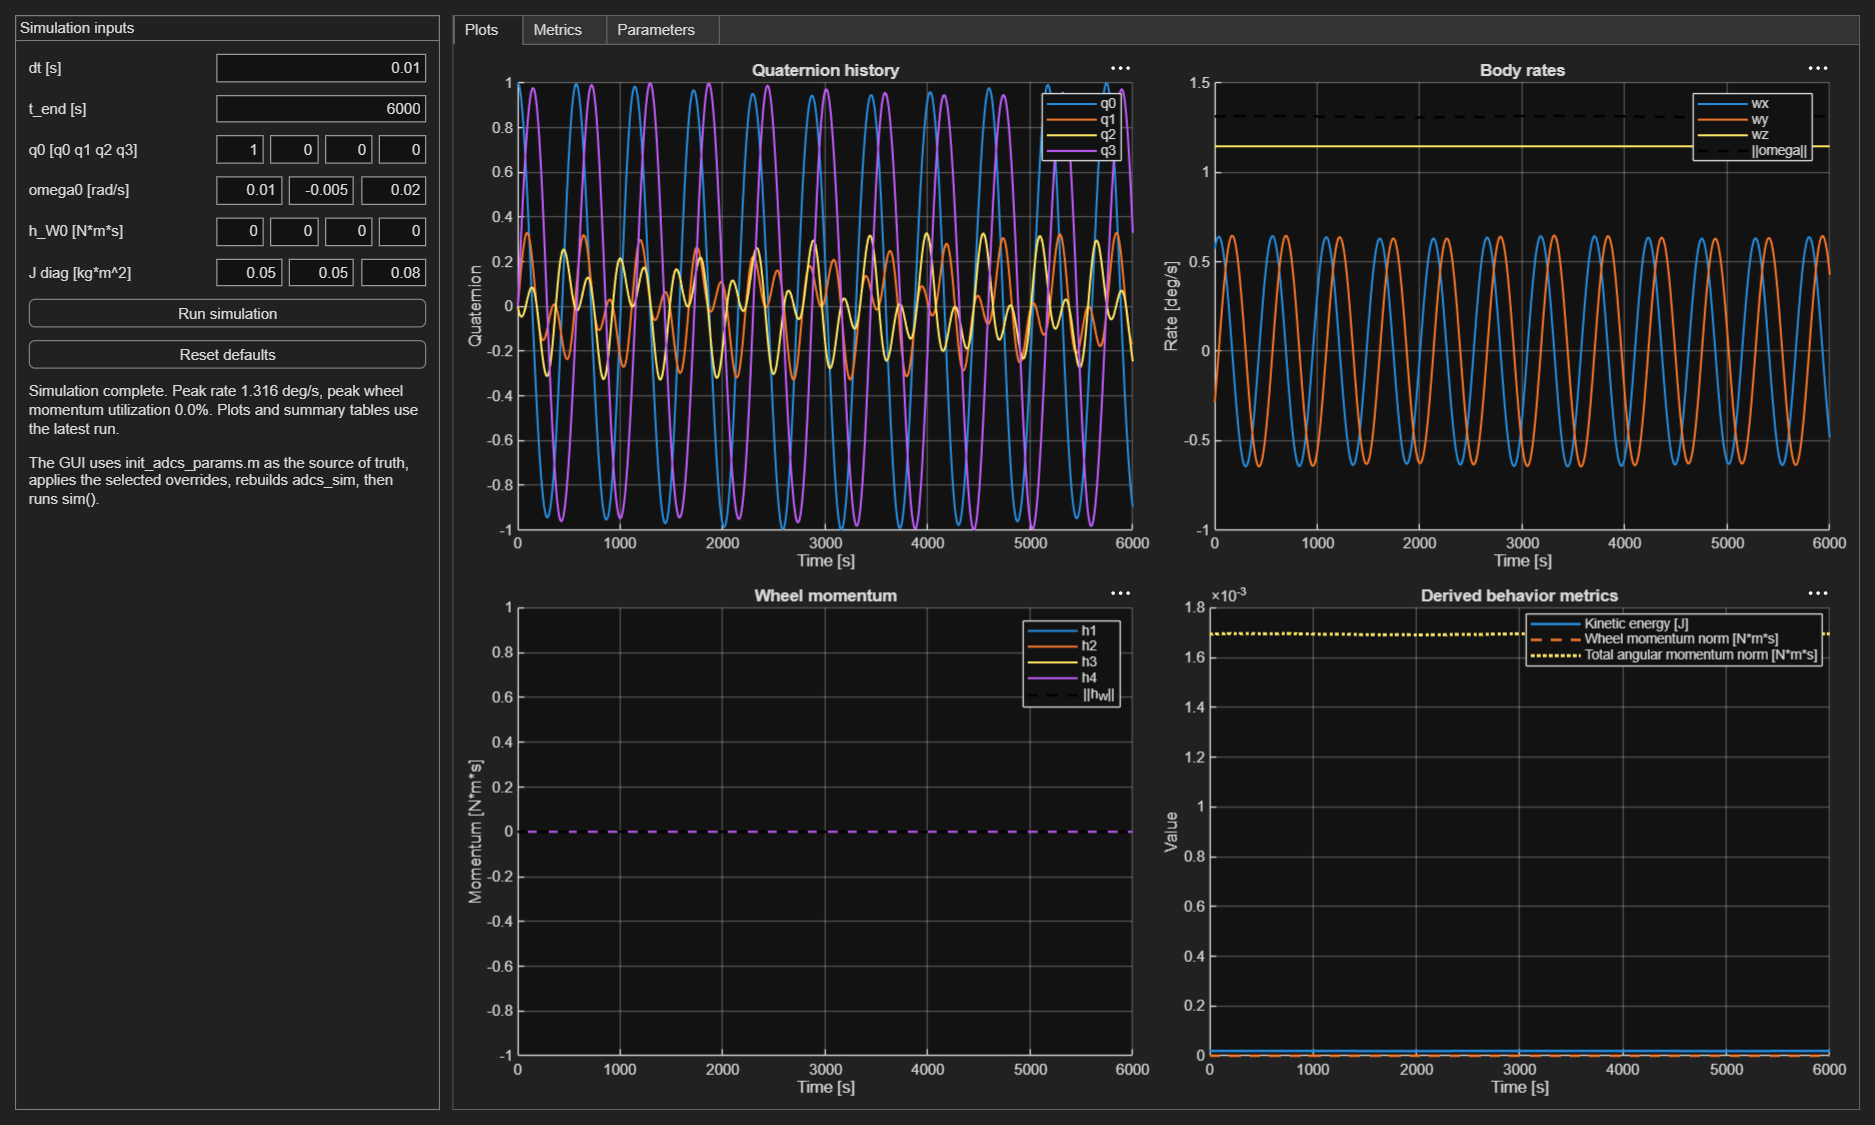
\includegraphics[width=\textwidth]{gui_results.png}
\caption{GUI after a simulation run. The plots tab visualizes quaternion, rate, and wheel-momentum histories, while the metrics and parameters tabs summarize the run numerically.}
\label{fig:gui-results}
\end{figure}

Figure \ref{fig:default-summary} shows a compact standalone summary plot exported from a default run.

\begin{figure}[H]
\centering
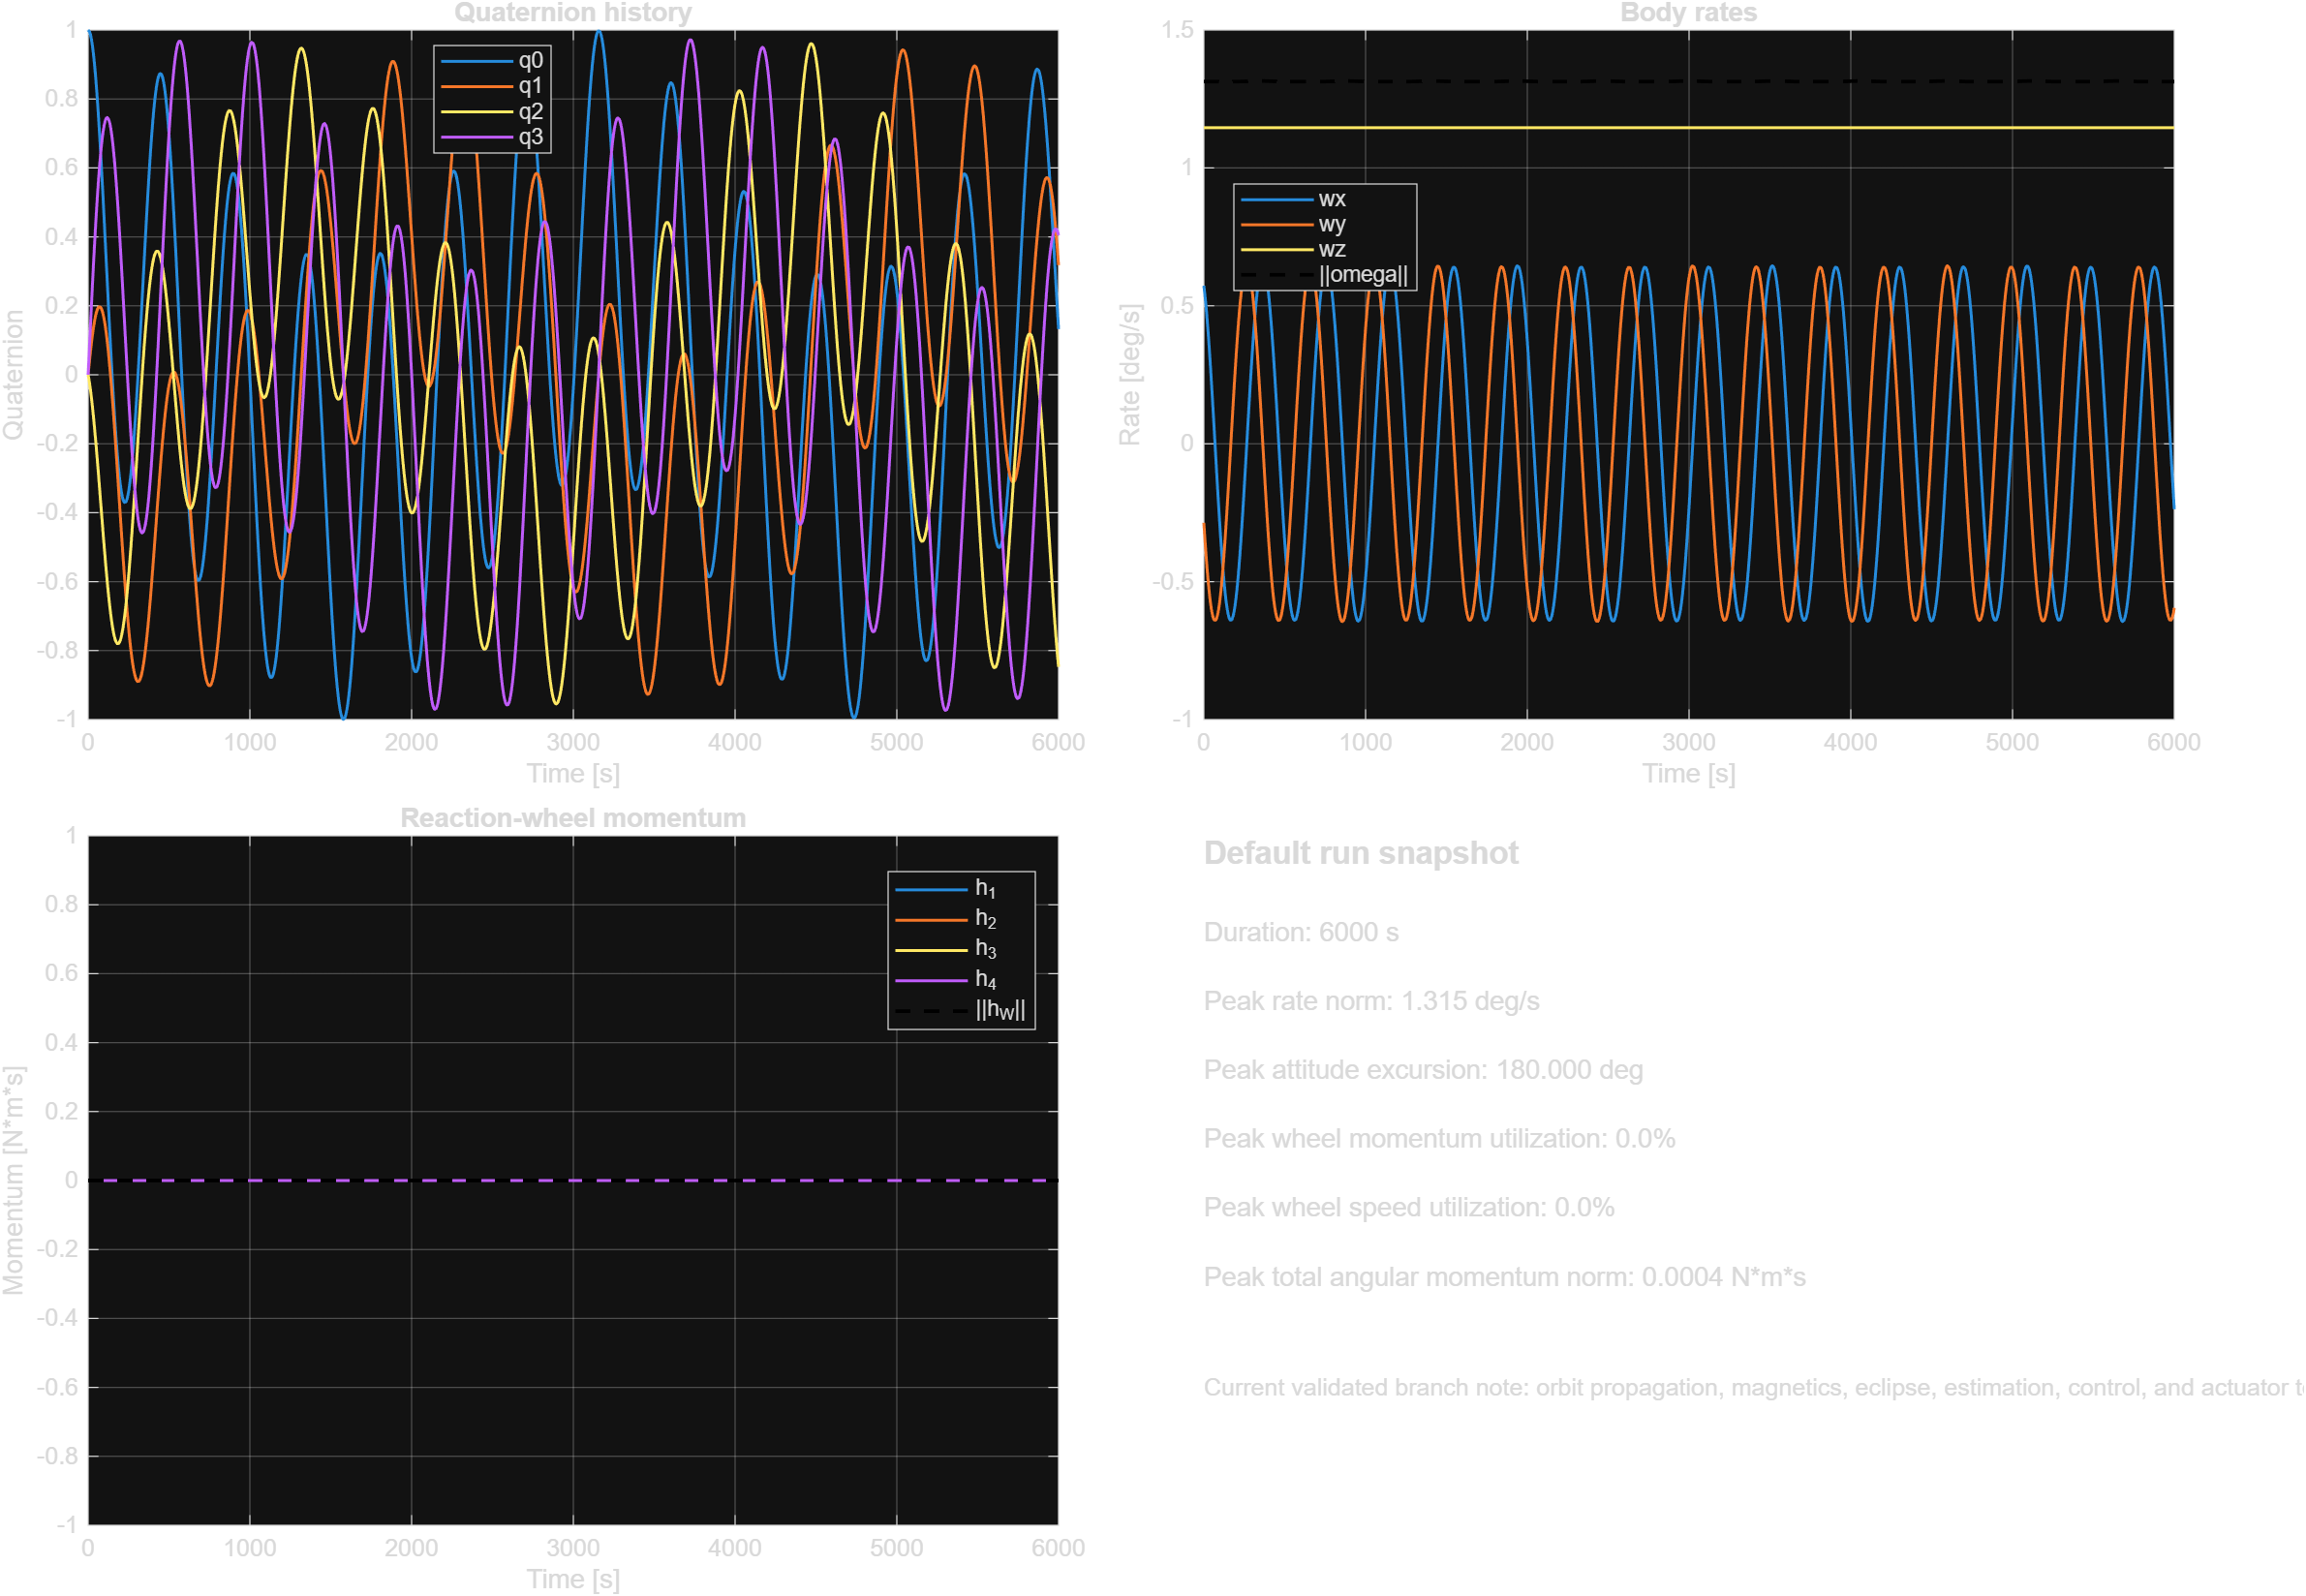
\includegraphics[width=\textwidth]{default_run_summary.png}
\caption{Default run summary exported from the repository. The current validated branch produces nontrivial attitude and rate histories, but zero wheel-momentum growth because the present actuator path is a zero-torque fallback.}
\label{fig:default-summary}
\end{figure}

\subsection{Default-run interpretation}

With the repository defaults, a baseline run produces approximately:

\begin{itemize}
\item duration: 6000 s
\item peak rate norm: about 1.315 deg/s
\item peak attitude excursion: about 180 deg
\item peak wheel momentum utilization: 0\%
\item peak wheel speed utilization: 0\%
\end{itemize}

Those numbers are internally consistent with the current branch: the rigid-body state evolves, but control and actuator fallbacks do not build wheel momentum or apply closed-loop stabilizing torques.

\section{Subsystem-by-Subsystem Guide}

\subsection{ENVIRONMENT}

Conceptually, ENVIRONMENT answers: ``What does space look like around the spacecraft right now?''

\textbf{Inputs and outputs.} It has no top-level truth-state inputs; it uses the simulation clock and workspace parameters. It outputs:

\begin{itemize}
\item \texttt{Sun\_vec\_ECI}
\item \texttt{Moon\_vec\_ECI}
\item \texttt{B\_ECI}
\item \texttt{pos\_ECI}
\item \texttt{vel\_ECI}
\item \texttt{eclipse\_flag}
\end{itemize}

\textbf{What the blocks are meant to represent.}

\begin{itemize}
\item \texttt{Ephemeris\_Truth}: truth-side Sun and Moon direction in ECI, interpolated from CSV.
\item \texttt{Orbit\_Propagator}: orbital state generation.
\item \texttt{Magnetic\_Field\_Model}: Earth field in ECI.
\item \texttt{Eclipse\_Model}: whether the spacecraft is illuminated.
\end{itemize}

\textbf{What the validated branch actually does.}

\begin{itemize}
\item \texttt{Ephemeris\_Truth} is active and interpolates Sun and Moon unit vectors from the CSV arrays.
\item \texttt{Orbit\_Propagator} is currently a fixed-state fallback returning constant position and velocity.
\item \texttt{Magnetic\_Field\_Model} is currently a constant-field fallback.
\item \texttt{Eclipse\_Model} is currently a constant-sunlit fallback.
\end{itemize}

That means the environment dataflow is correct, but the present numerical fidelity is uneven.

\subsection{SENSORS}

Conceptually, SENSORS answers: ``Given the true spacecraft state and the environment, what would the onboard sensors report?''

\textbf{Inputs.}

\begin{itemize}
\item true attitude quaternion \texttt{q\_in}
\item true angular rate \texttt{omega\_in}
\item inertial Sun vector, Moon vector, magnetic field
\item eclipse flag
\item inertial position and velocity
\end{itemize}

\textbf{Outputs.}

\begin{itemize}
\item \texttt{q\_meas}
\item \texttt{omega\_meas}
\item \texttt{sun\_meas}
\item \texttt{B\_body\_meas}
\item \texttt{pos\_meas}
\item \texttt{vel\_meas}
\end{itemize}

\textbf{What is physically active right now.}

\begin{itemize}
\item \texttt{Sun\_Sensor\_Suite} rotates the inertial Sun vector into the body frame and zeros it when eclipse is active.
\item \texttt{Magnetometer} rotates the inertial magnetic-field vector into the body frame.
\end{itemize}

\textbf{What is currently simplified.}

\begin{itemize}
\item \texttt{Star\_Tracker} is a quaternion passthrough fallback.
\item \texttt{IMU} is an angular-rate passthrough fallback.
\item \texttt{GNSS\_Position} and \texttt{GNSS\_Velocity} are position and velocity passthrough fallbacks.
\end{itemize}

So, in the present branch, SENSORS is best understood as a mixed ``real transform plus passthrough'' layer.

\subsection{CONTROL}

Conceptually, CONTROL answers: ``Given measurements and mission logic, what should the spacecraft command next?''

\textbf{Inputs.}

\begin{itemize}
\item measured attitude and angular rate
\item measured Sun vector and magnetic field in the body frame
\item measured position and velocity
\item current reaction-wheel momentum state
\end{itemize}

\textbf{Outputs.}

\begin{itemize}
\item reaction-wheel torque command
\item magnetorquer dipole command
\item CMG gimbal command
\end{itemize}

\textbf{Architectural role of each block.}

\begin{itemize}
\item \texttt{Onboard\_Ephemeris}: controller-side environmental prediction.
\item \texttt{Attitude\_Estimator}: estimated quaternion and rate.
\item \texttt{Reference\_Generator}: desired pointing and desired angular rate.
\item \texttt{Mode\_Manager}: detumble / coarse / fine pointing logic.
\item \texttt{Control\_Law}: mapping from estimated state and reference to actuator commands.
\end{itemize}

\textbf{Validated-branch behavior.}

\begin{itemize}
\item \texttt{Onboard\_Ephemeris} outputs constant reference vectors.
\item \texttt{Attitude\_Estimator} normalizes \texttt{q\_meas}, forces a positive scalar sign convention, and passes through \texttt{omega\_meas}.
\item \texttt{Reference\_Generator} returns an identity quaternion and zero desired rate.
\item \texttt{Mode\_Manager} returns a constant mode identifier of 2.
\item \texttt{Control\_Law} outputs zero commands for all actuators.
\end{itemize}

This means CONTROL is presently carrying the \emph{interface contract} of a flight control stack, but not yet the intended flight-quality control behavior described in the domain notes.

\subsection{ACTUATORS}

Conceptually, ACTUATORS answers: ``How do commanded actuator actions become torques or momentum changes in the body?''

\textbf{Inputs.}

\begin{itemize}
\item reaction-wheel torque command
\item magnetorquer dipole command
\item CMG gimbal command
\item measured body-frame magnetic field
\end{itemize}

\textbf{Outputs.}

\begin{itemize}
\item \texttt{ext\_torque}
\item \texttt{rw\_torque\_body}
\item \texttt{rw\_tau\_wheels}
\end{itemize}

\textbf{Why there are three outputs instead of one.}

This is an important reading detail. The model separates:

\begin{itemize}
\item external body torque from MTQ and CMG,
\item reaction-wheel torque applied to the spacecraft body,
\item wheel-axis torques that integrate into the wheel-momentum state.
\end{itemize}

That is good modeling structure, because reaction wheels do not just apply a body torque; they also change the wheels' internal stored angular momentum.

\textbf{Validated-branch behavior.}

All three actuator blocks are currently zero-output fallbacks. As a result:

\begin{itemize}
\item \texttt{ext\_torque} is zero,
\item \texttt{rw\_torque\_body} is zero,
\item \texttt{rw\_tau\_wheels} is zero.
\end{itemize}

This is why the default run shows zero wheel-momentum buildup and zero wheel-speed utilization.

\subsection{DYNAMICS}

Conceptually, DYNAMICS answers: ``Given the current torques and internal momentum state, how does the spacecraft rotate next?''

\textbf{Inputs.}

\begin{itemize}
\item commanded external torque
\item reaction-wheel body torque
\item reaction-wheel wheel-axis torques
\item position, velocity, Sun vector, eclipse flag, magnetic field
\end{itemize}

\textbf{Outputs.}

\begin{itemize}
\item \texttt{q\_out}
\item \texttt{omega\_out}
\item \texttt{h\_W\_out}
\end{itemize}

\textbf{Physically active blocks in the validated branch.}

\begin{itemize}
\item \texttt{Euler\_RHS}
\item \texttt{Gravity\_Gradient}
\item \texttt{Quat\_RHS}
\item \texttt{Quat\_Norm}
\item the \texttt{Integ\_omega}, \texttt{Integ\_hW}, and \texttt{Integ\_q} integrators
\end{itemize}

\textbf{Currently simplified blocks.}

\begin{itemize}
\item \texttt{Aero\_Drag\_Torque}
\item \texttt{SRP\_Torque}
\item \texttt{Residual\_Mag\_Torque}
\end{itemize}

\textbf{Why DYNAMICS is the heart of the current branch.}

Even with the simplified control and actuator layers, DYNAMICS still integrates a genuine rigid-body rotational system with quaternion kinematics and gravity-gradient torque. That is why the default run still produces a changing quaternion and changing angular-rate history.

\section{Physics and Math Background for Hard-to-Read Parts}

This section is intentionally short and practical. It is not a full ADCS textbook; it is the minimum background a beginner needs to decode the model.

\subsection{Frames}

The repository primarily uses:

\begin{itemize}
\item \textbf{ECI} for inertial quantities such as Sun direction, magnetic field, position, and velocity.
\item \textbf{Body frame} for spacecraft-fixed quantities such as body rates, body torque, sensor boresights, and actuator axes.
\end{itemize}

Whenever you see a block that rotates a vector from ECI to body, it is answering the question: ``What does this inertial direction look like from the spacecraft's own point of view?''

\subsection{Quaternions}

The quaternion convention is scalar-first:

\[
q = [q_0,\ q_1,\ q_2,\ q_3]^T
\]

with unit norm:

\[
\|q\| = 1
\]

The quaternion derivative block uses:

\[
\dot{q} = \frac{1}{2}\Omega(\omega)q
\]

where the matrix in the code corresponds to the scalar-first convention. The model then renormalizes the quaternion after integration so numerical drift does not slowly violate the unit-norm constraint.

\subsection{Rigid-body rotational dynamics}

The core rotational equation implemented in \texttt{Euler\_RHS} is:

\[
\dot{\omega} = J^{-1}\left(\tau_{\text{ext}} - \omega \times H_{\text{total}} - \tau_{\text{rw,body}}\right)
\]

with

\[
H_{\text{total}} = J\omega + A_W h_W
\]

This is a strong clue that the model is trying to keep track of both:

\begin{itemize}
\item the spacecraft body's angular momentum, and
\item the stored angular momentum in the reaction wheels.
\end{itemize}

With the current default parameter set, the inertia tensor is the uniform-density baseline implied by the declared 4 kg, \(0.10 \times 0.10 \times 0.30\) m bus geometry:

\[
J = \mathrm{diag}([0.0333,\ 0.0333,\ 0.0067]) \ \text{kg·m}^2
\]

\subsection{Gravity-gradient torque}

The gravity-gradient block computes the classic body-frame disturbance torque:

\[
\tau_{gg} = \frac{3\mu}{R^3}\left(r_{\text{body}} \times J r_{\text{body}}\right)
\]

Physically, this is the torque that appears because different parts of an extended spacecraft feel slightly different gravitational pull when the body is not inertially isotropic. In the current validated branch, the quaternion-to-DCM mapping used here matches the same ECI-to-body convention used by the active Sun-sensor and magnetometer transforms.

\subsection{Magnetorquer torque}

The intended magnetorquer relation is:

\[
\tau = m \times B
\]

where \(m\) is the commanded dipole moment and \(B\) is the local magnetic field in the body frame. The current validated branch preserves this interface, even though the present actuator block is a fallback.

\subsection{Reaction-wheel momentum}

Reaction wheels are internal actuators. They do not create net system angular momentum out of nothing; they exchange angular momentum between the wheel rotors and the spacecraft body. That is why the model tracks wheel momentum \(h_W\) separately and feeds it both into DYNAMICS and CONTROL.

\section{Detailed End-to-End Data Path}

This section answers the user-level question: ``How does data actually move from environment to workspace?''

\subsection{Step 1: Environment truth is assembled}

At each simulation time, ENVIRONMENT produces:

\begin{itemize}
\item Sun direction in ECI from interpolated ephemeris
\item Moon direction in ECI from interpolated ephemeris
\item spacecraft position and velocity
\item Earth magnetic field in ECI
\item eclipse status
\end{itemize}

\subsection{Step 2: Sensors reinterpret truth as measurements}

SENSORS consumes truth attitude and rate from DYNAMICS and truth environment signals from ENVIRONMENT. It then emits:

\begin{itemize}
\item measured quaternion
\item measured rate
\item body-frame Sun vector
\item body-frame magnetic field
\item measured position and velocity
\end{itemize}

In the current branch, the Sun and magnetometer transformations are active, while several other sensors are passthrough fallbacks.

\subsection{Step 3: Control decides what to command}

CONTROL takes those measurements and the wheel-momentum state, then forms:

\begin{itemize}
\item desired reference attitude and rate
\item current mode
\item actuator commands
\end{itemize}

In the present branch this stage is structurally present but numerically simplified: the reference is fixed, mode is fixed, and commanded torques are zero.

\subsection{Step 4: Actuators map commands into torque channels}

ACTUATORS separates the results into:

\begin{itemize}
\item body torque from non-wheel actuators
\item body torque from wheel reaction
\item wheel-axis torques for wheel momentum integration
\end{itemize}

This separation is conceptually important even though the current fallback outputs are zero.

\subsection{Step 5: Dynamics propagates the state}

DYNAMICS sums commanded and disturbance torques, computes angular acceleration, integrates angular rate and quaternion, integrates wheel momentum, and emits:

\begin{itemize}
\item normalized attitude quaternion
\item body angular rate
\item wheel momentum state
\end{itemize}

\subsection{Step 6: Logs and GUI summarize the run}

The model sends:

\begin{itemize}
\item \texttt{q\_out} to \texttt{Q\_To\_Workspace} as \texttt{q\_log}
\item \texttt{omega\_out} to \texttt{Omega\_To\_Workspace} as \texttt{omega\_log}
\item \texttt{h\_W\_out} to \texttt{HW\_To\_Workspace} as \texttt{h\_W\_log}
\end{itemize}

Then \texttt{summarize\_adcs\_simulation.m} turns those logs into the metrics shown in the GUI.

\section{What a Beginner Should Notice First in Each Screenshot}

\subsection{Top-level model}

When you open the top-level model, do not try to follow every line at once. First answer only four questions:

\begin{enumerate}
\item What are the five major subsystems?
\item Which signals move left to right?
\item Which signals feed back from DYNAMICS?
\item Which outputs are logged to the workspace?
\end{enumerate}

Once you can answer those, the whole model stops looking like a random wire jungle.

\subsection{GUI}

When you open the GUI, look for:

\begin{enumerate}
\item the left column of editable run inputs
\item the run and reset buttons
\item the status text telling you what the GUI will do
\item the tabs on the right: plots, metrics, parameters
\end{enumerate}

That is the whole interaction model.

\section{Current Validated Branch: Accuracy and Limitations}

It is important not to overstate what the current branch is doing.

\subsection{What is meaningfully modeled now}

\begin{itemize}
\item quaternion kinematics
\item rigid-body rotational dynamics
\item gravity-gradient torque
\item transformation of inertial Sun and magnetic vectors into the body frame
\item logging and derived-metric computation
\end{itemize}

\subsection{What is structurally present but currently simplified}

\begin{itemize}
\item orbit propagation
\item Earth magnetic-field modeling
\item eclipse logic
\item star tracker, IMU, and GNSS noise and sample logic
\item onboard ephemeris
\item attitude estimation beyond simple normalization
\item reference generation
\item mode logic
\item control torque generation
\item reaction-wheel, magnetorquer, and CMG torque realization
\item aerodynamic drag torque
\item solar radiation pressure torque
\item residual magnetic dipole torque
\end{itemize}

\subsection{How to phrase the model honestly}

The fairest one-sentence description of the repository today is:

\begin{quote}
The project already contains a well-structured closed-loop ADCS Simulink architecture with physically meaningful attitude-state propagation, but several environment, estimation, control, and actuator blocks are still running compile-safe fallback implementations in the validated branch.
\end{quote}

That statement is much more accurate than simply calling the current branch a fully high-fidelity orbital behavior simulator.

\section{Quick Reference}

\subsection{Acronyms}

\begin{table}[H]
\centering
\begin{tabularx}{\textwidth}{@{}lY@{}}
\toprule
\textbf{Acronym} & \textbf{Meaning} \\
\midrule
ADCS & Attitude Determination and Control System \\
ECI & Earth-Centered Inertial frame \\
FSS & Fine Sun Sensor \\
GNSS & Global Navigation Satellite System receiver \\
GUI & Graphical User Interface \\
IMU & Inertial Measurement Unit \\
MEKF & Multiplicative Extended Kalman Filter \\
MTQ & Magnetorquer \\
PD & Proportional-Derivative \\
RW & Reaction Wheel \\
SRP & Solar Radiation Pressure \\
TRIAD & Two-vector deterministic attitude determination method \\
\bottomrule
\end{tabularx}
\caption{Acronyms used throughout the model and this guide.}
\end{table}

\subsection{Fast reading checklist}

If you only have ten minutes with the project, inspect these in order:

\begin{enumerate}
\item \texttt{README.md}
\item \texttt{reference.md}
\item \texttt{build\_adcs\_model.m}
\item top-level Simulink diagram
\item \texttt{init\_adcs\_params.m}
\item \texttt{launch\_adcs\_gui.m}
\item \texttt{builders/build\_dynamics.m}
\end{enumerate}

\appendix

\section{Subsystem Screenshot Gallery}

\begin{landscape}
\begin{figure}[p]
\centering
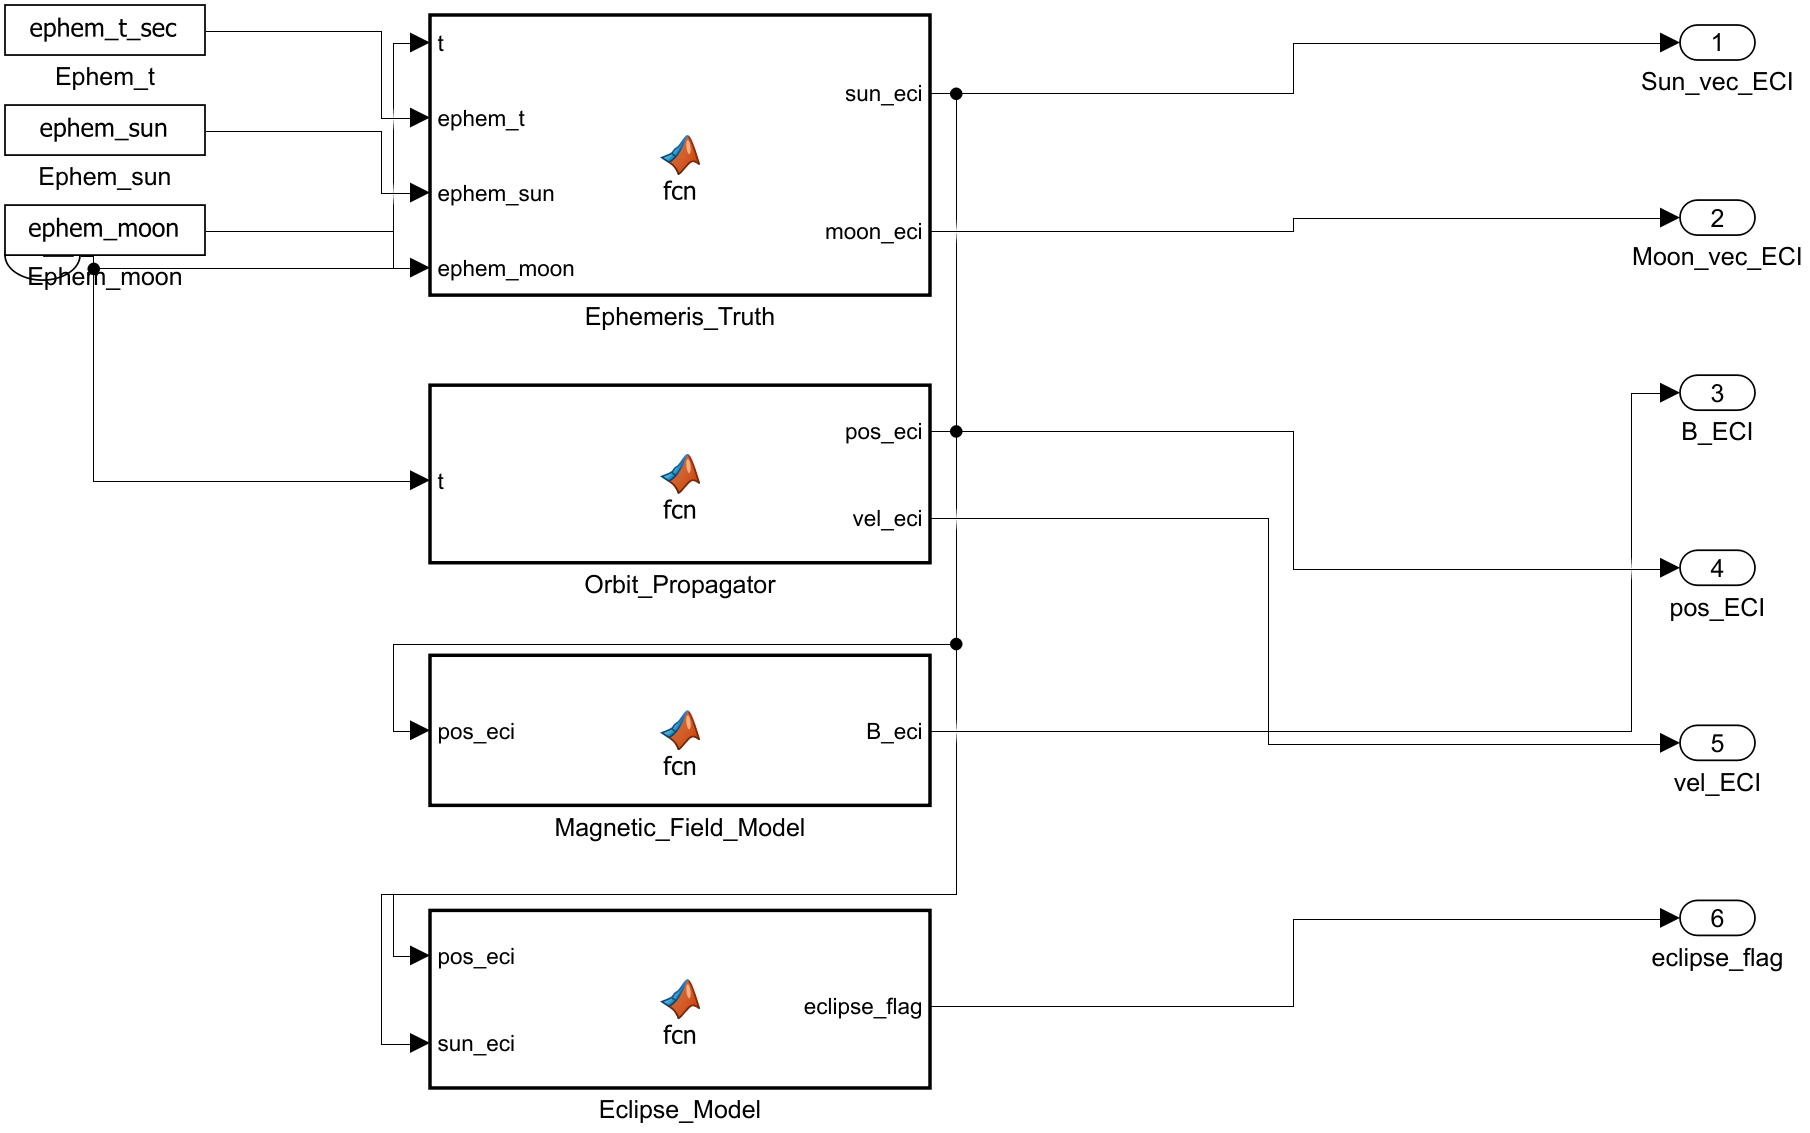
\includegraphics[width=0.95\linewidth]{environment_subsystem.png}
\caption{ENVIRONMENT subsystem. Start here when you want to understand where the truth-side Sun, Moon, orbit, magnetic field, and eclipse signals come from.}
\end{figure}
\end{landscape}

\begin{landscape}
\begin{figure}[p]
\centering
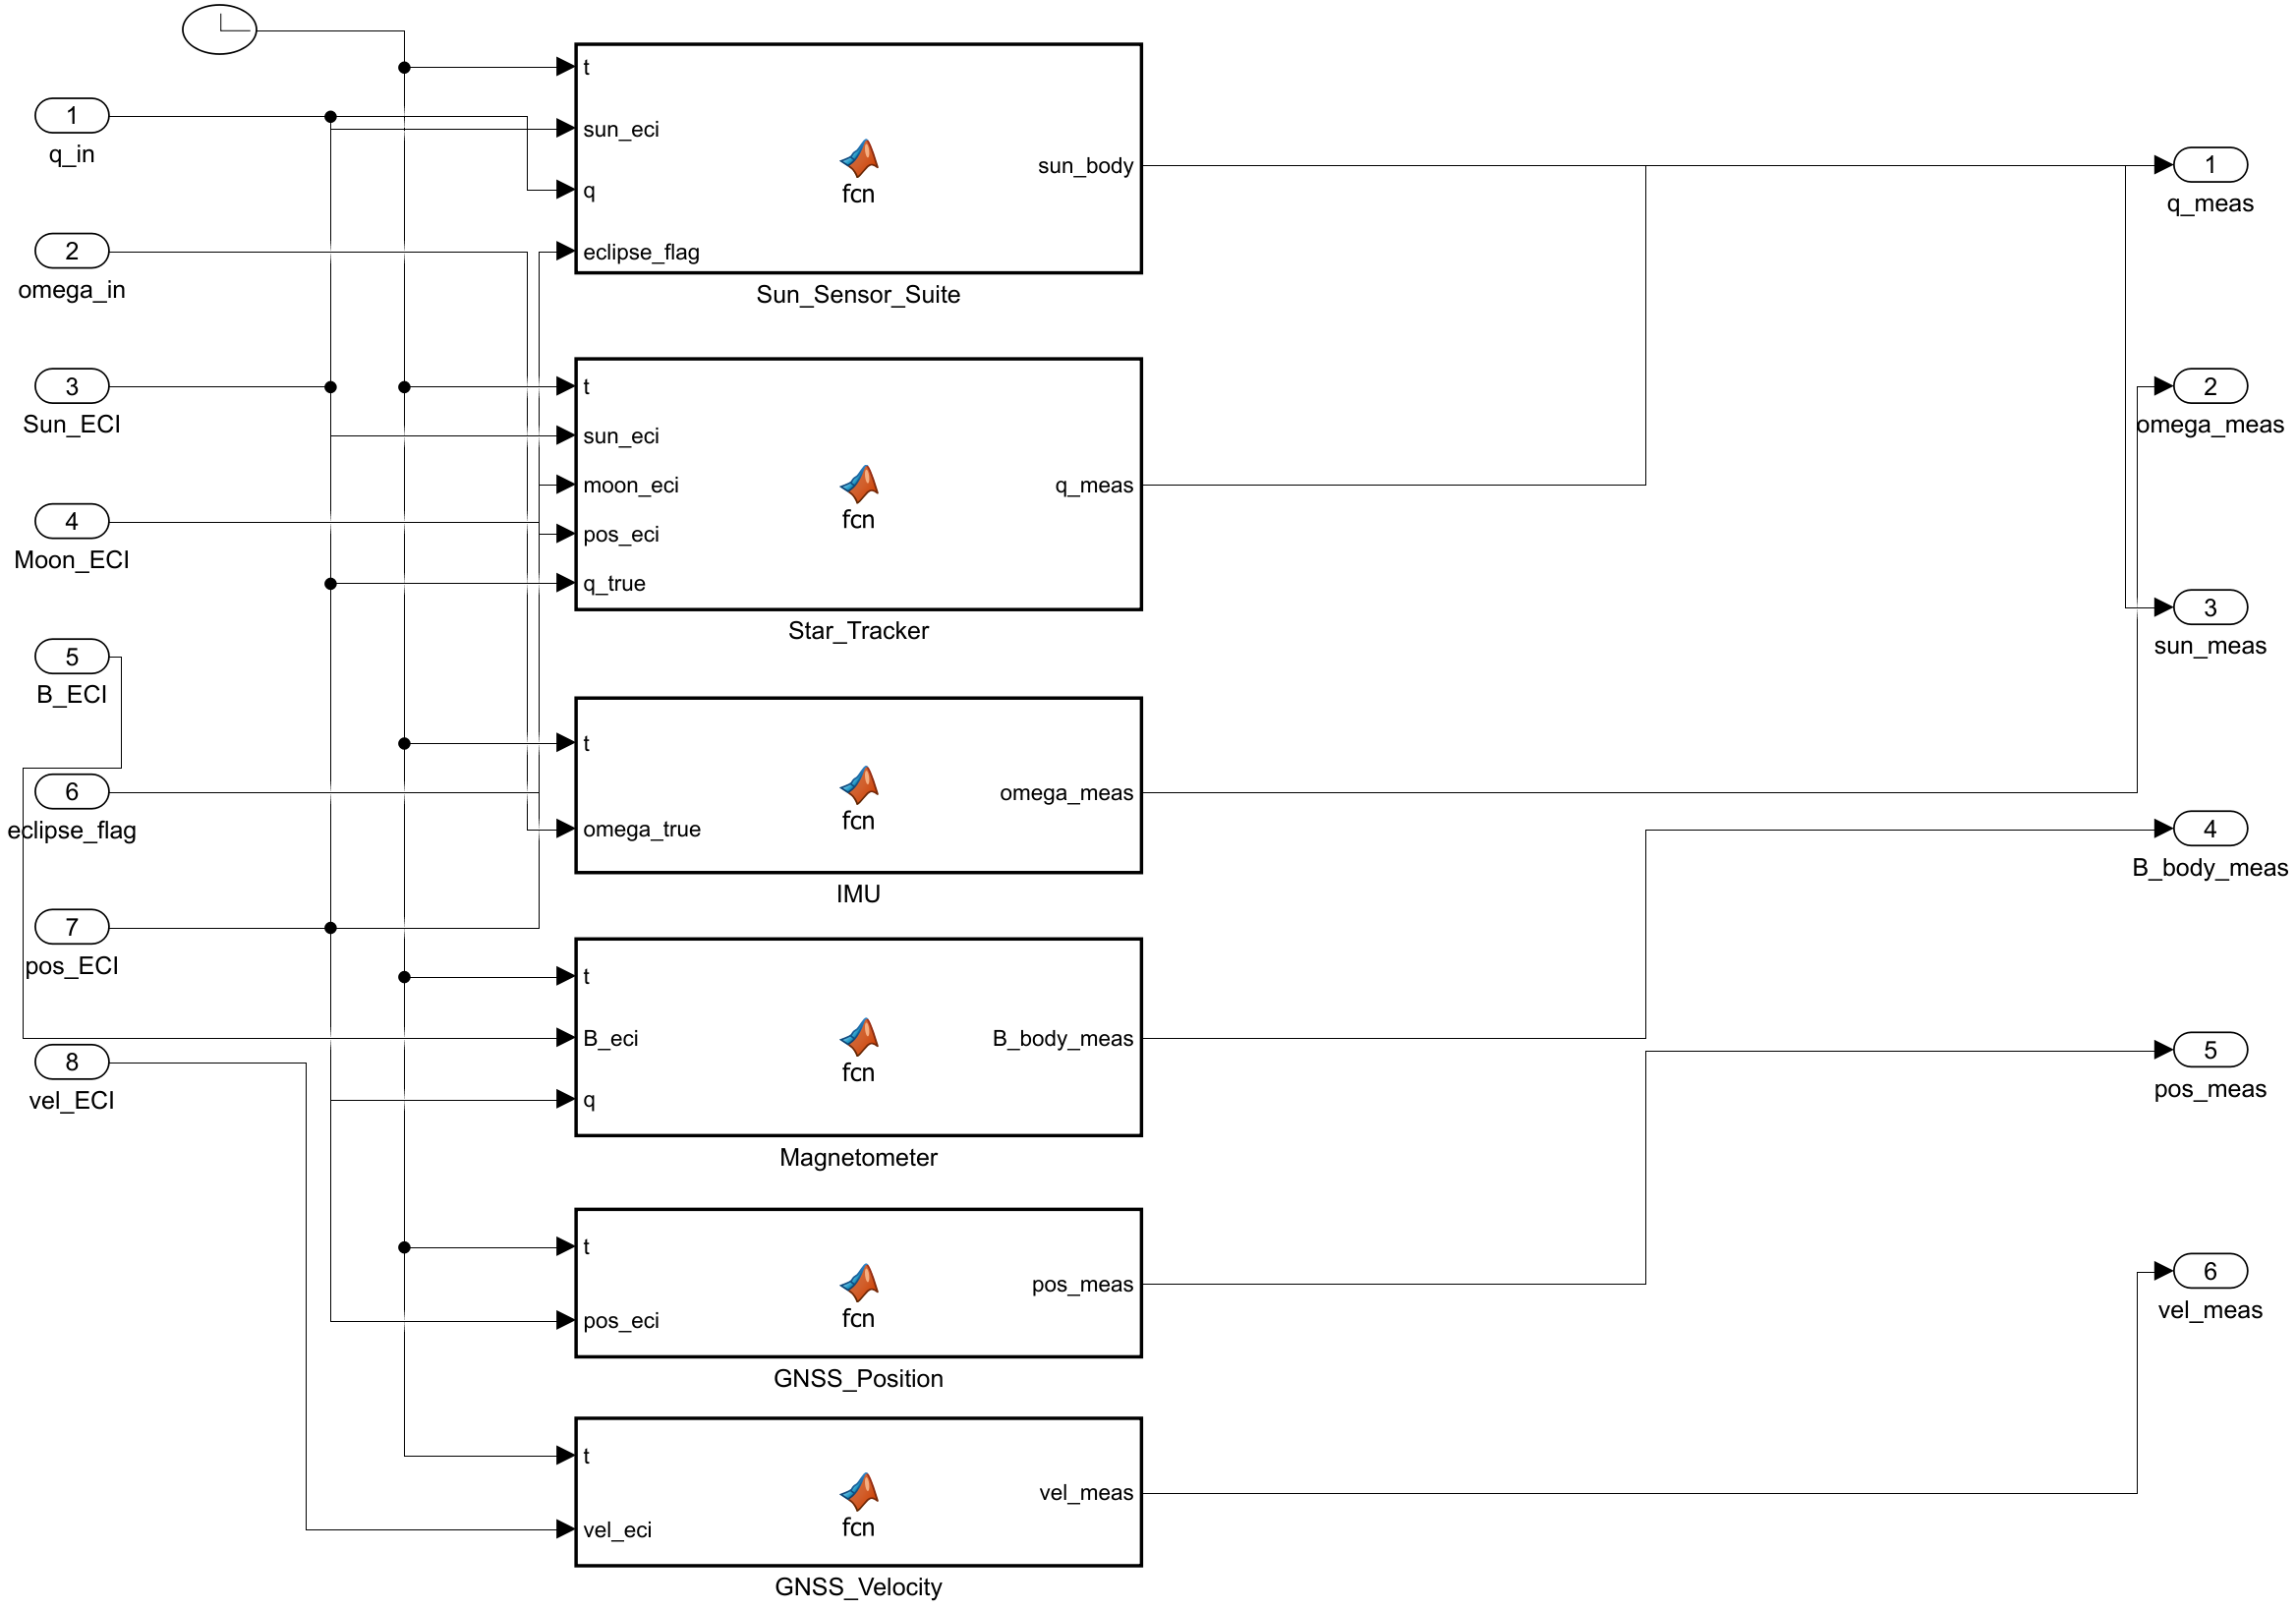
\includegraphics[width=0.95\linewidth]{sensors_subsystem.png}
\caption{SENSORS subsystem. This is where true state and environment are turned into measurements.}
\end{figure}
\end{landscape}

\begin{landscape}
\begin{figure}[p]
\centering
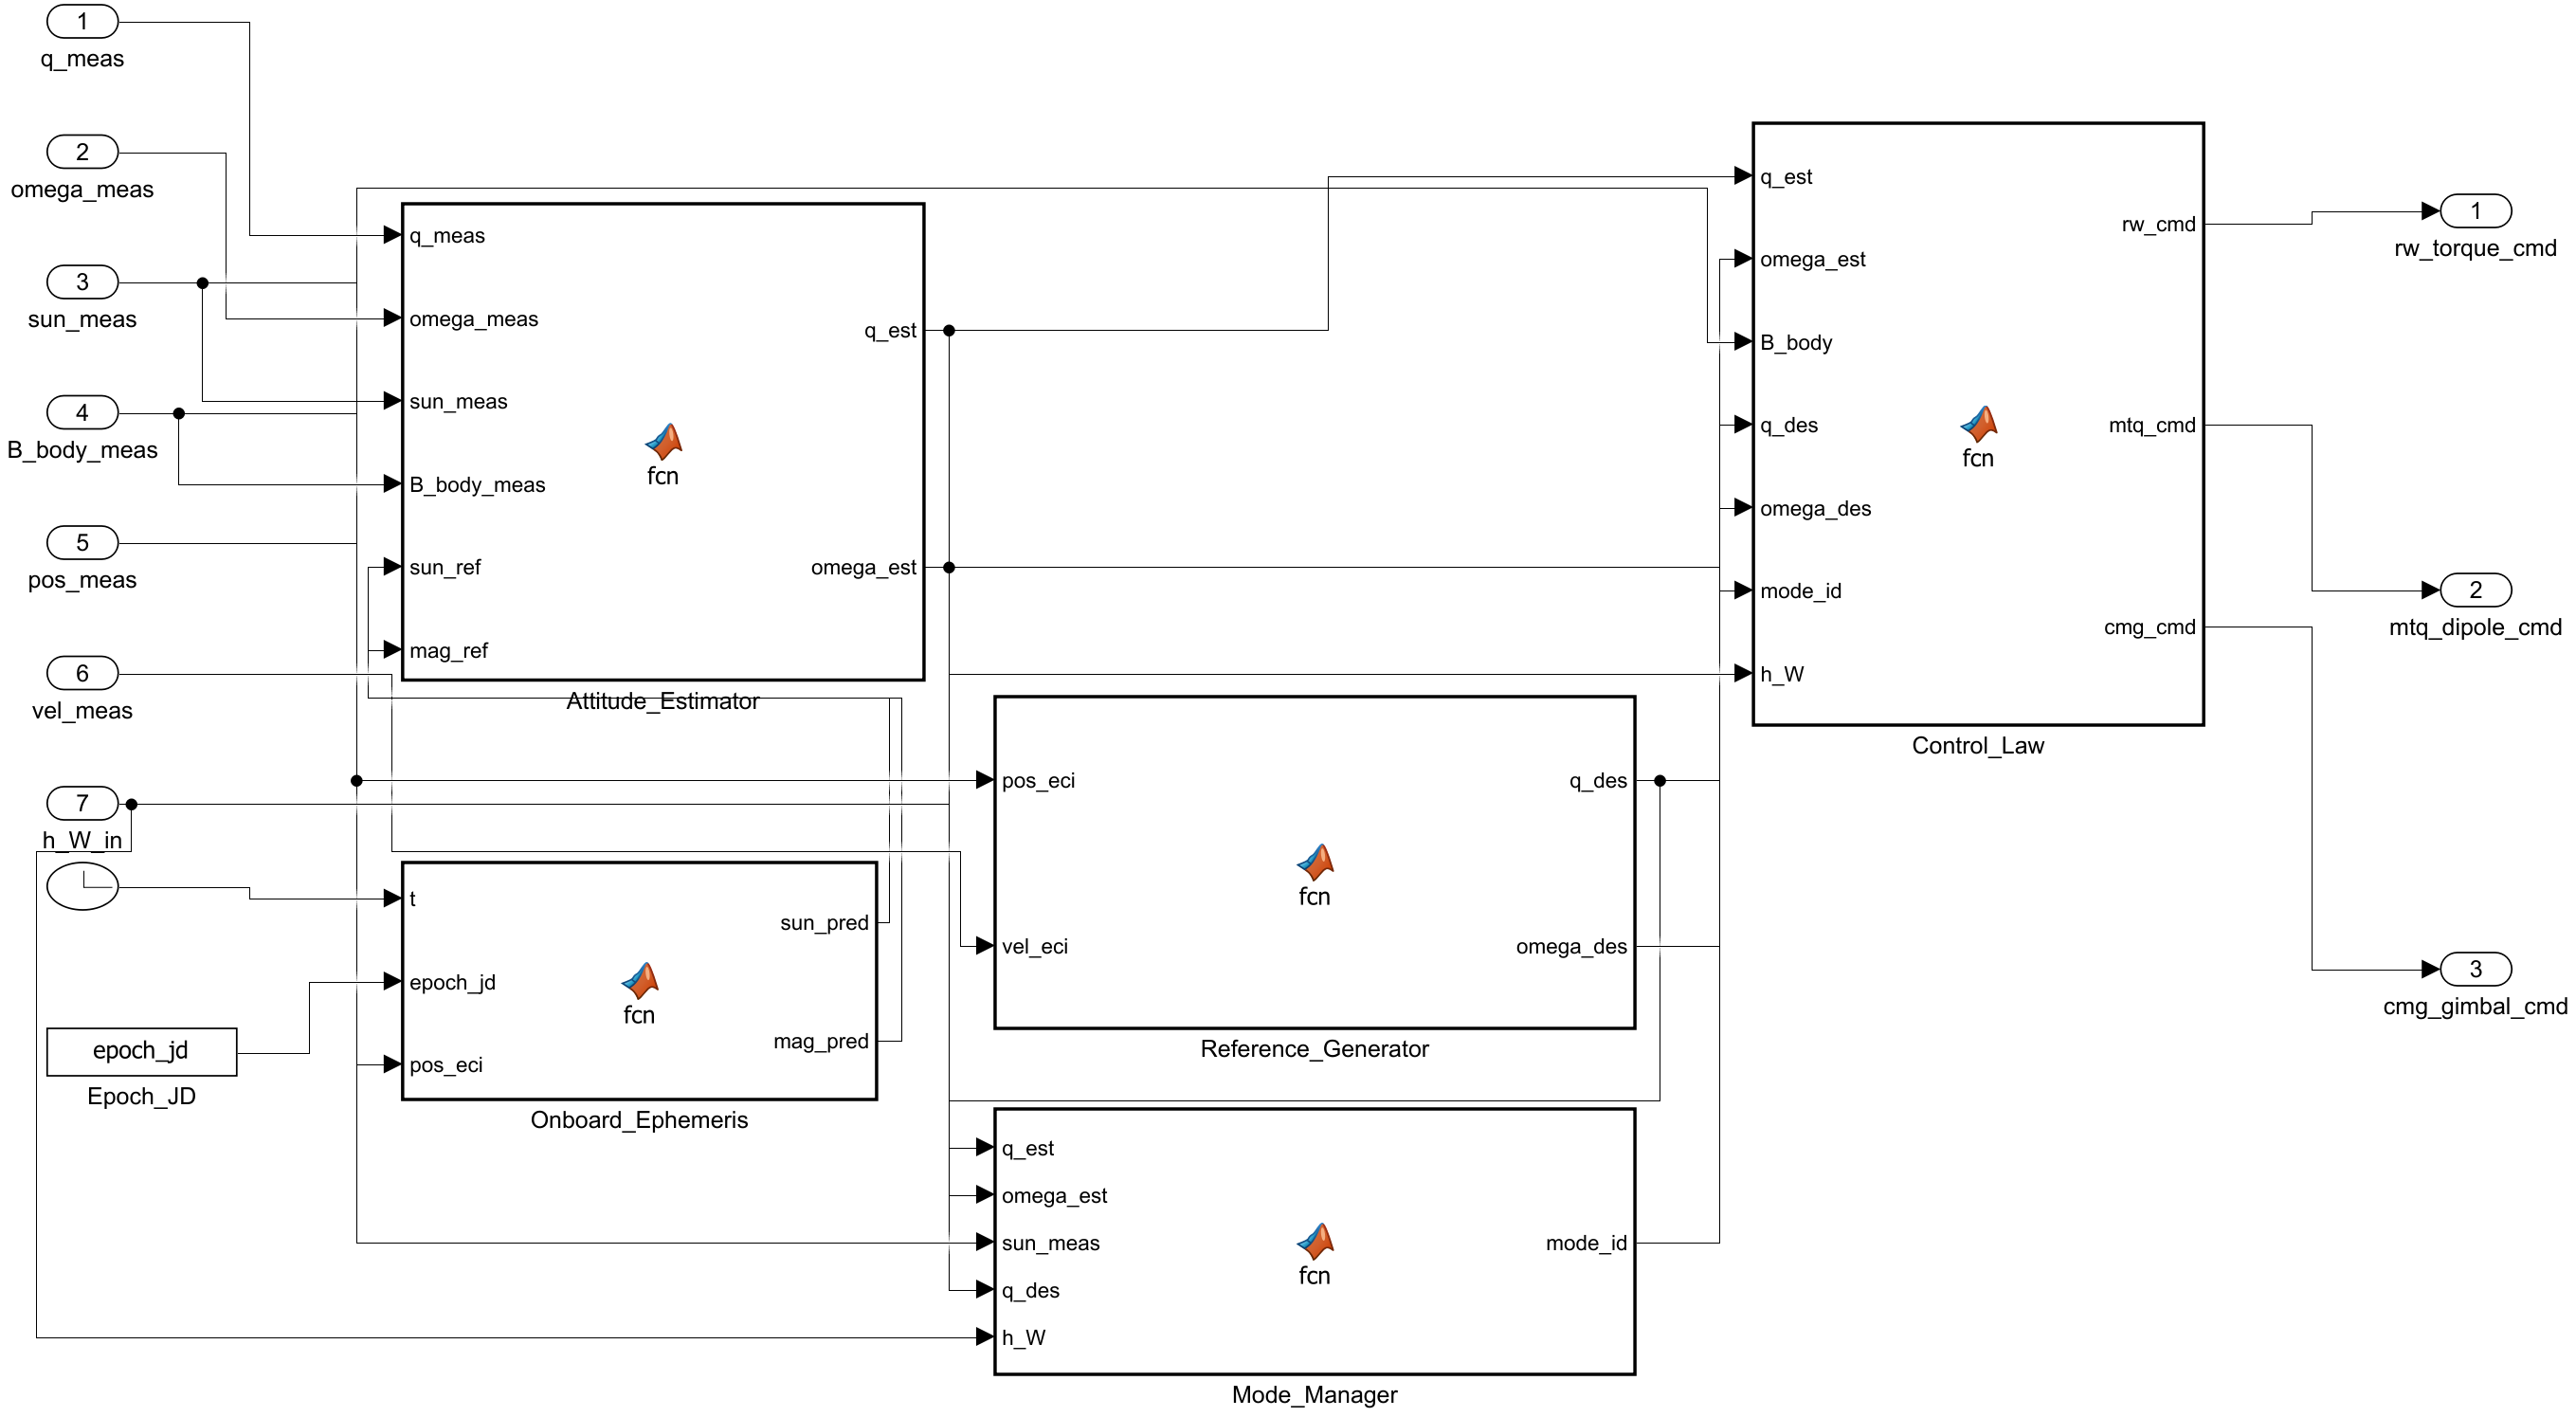
\includegraphics[width=0.95\linewidth]{control_subsystem.png}
\caption{CONTROL subsystem. The current branch preserves the full interface structure even though several blocks are simplified fallbacks.}
\end{figure}
\end{landscape}

\begin{landscape}
\begin{figure}[p]
\centering
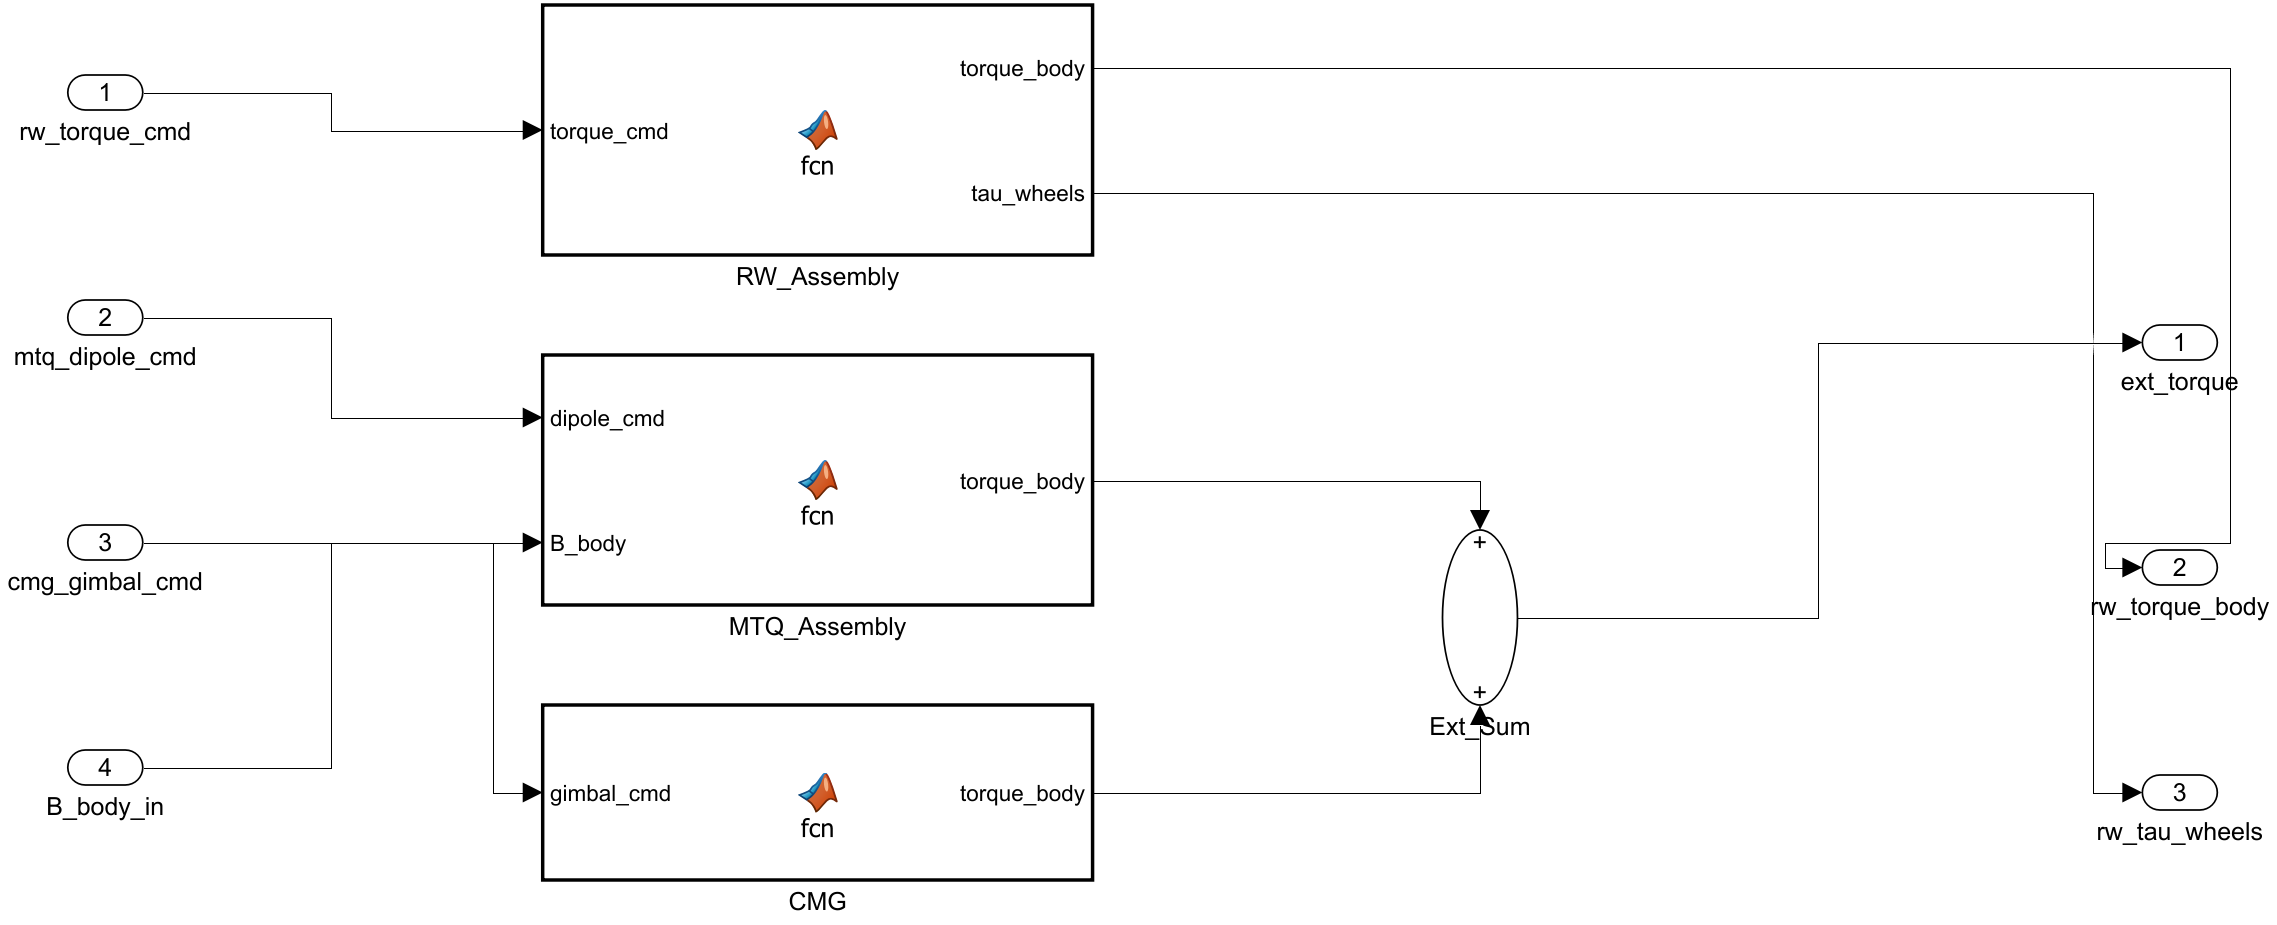
\includegraphics[width=0.95\linewidth]{actuators_subsystem.png}
\caption{ACTUATORS subsystem. Note the intentional split between external torque, wheel-body torque, and wheel-axis torque.}
\end{figure}
\end{landscape}

\begin{landscape}
\begin{figure}[p]
\centering
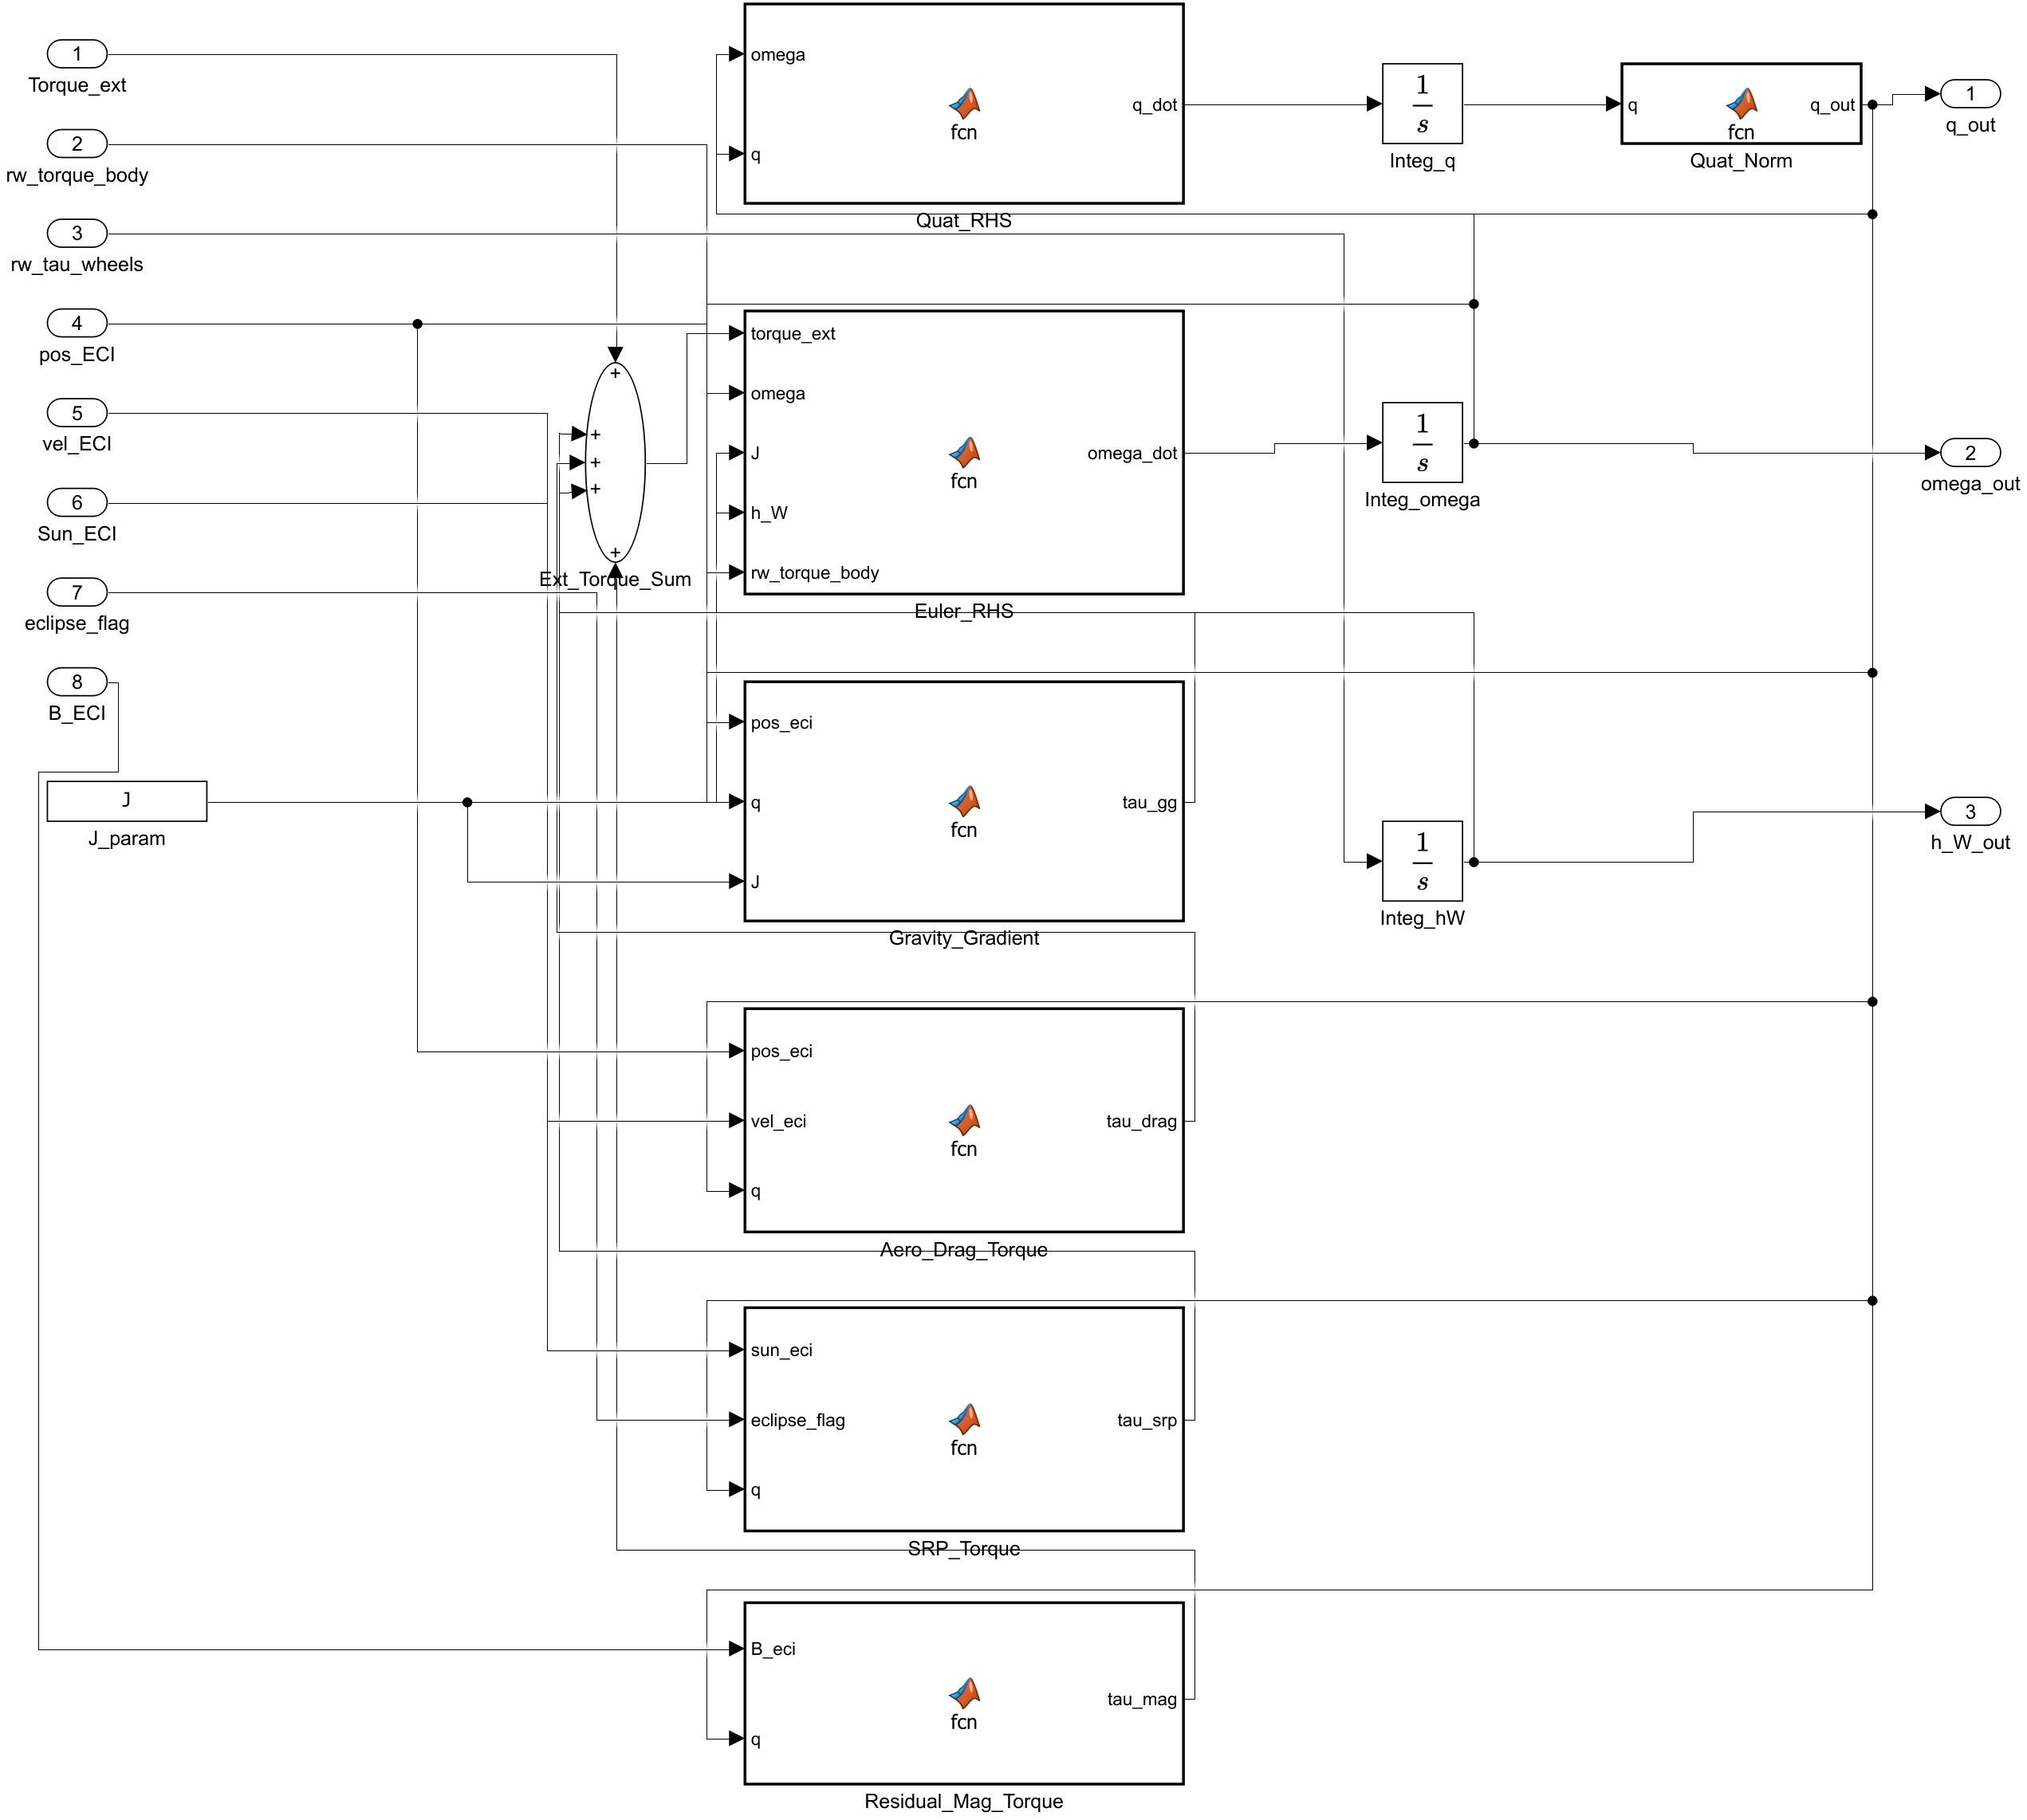
\includegraphics[width=0.75\linewidth]{dynamics_subsystem.png}
\caption{DYNAMICS subsystem. This is the core of the current validated branch and the main place to study quaternion propagation, torque summation, and rigid-body state integration.}
\end{figure}
\end{landscape}

\section{Sources and Further Reading}

\subsection*{Repository sources}
\addcontentsline{toc}{subsection}{Sources and Further Reading}

\begin{itemize}
\item \texttt{README.md}
\item \texttt{reference.md}
\item \texttt{init\_adcs\_params.m}
\item \texttt{build\_adcs\_model.m}
\item \texttt{builders/build\_environment.m}
\item \texttt{builders/build\_sensors.m}
\item \texttt{builders/build\_control.m}
\item \texttt{builders/build\_actuators.m}
\item \texttt{builders/build\_dynamics.m}
\item \texttt{launch\_adcs\_gui.m}
\item \texttt{simulate\_adcs\_case.m}
\item \texttt{summarize\_adcs\_simulation.m}
\item \texttt{skills.md}
\end{itemize}

\subsection*{External ADCS and modeling references}

\begin{itemize}
\item F. Landis Markley and John L. Crassidis, \textit{Fundamentals of Spacecraft Attitude Determination and Control}. Springer, 2014.
\item Hanspeter Schaub and John L. Junkins, \textit{Analytical Mechanics of Space Systems}. AIAA.
\item Howard D. Curtis, \textit{Orbital Mechanics for Engineering Students}. Elsevier.
\item Marcel J. Sidi, \textit{Spacecraft Dynamics and Control}. Cambridge University Press.
\item Oliver Montenbruck and Eberhard Gill, \textit{Satellite Orbits}. Springer.
\item MathWorks documentation for Simulink subsystem wiring, Scope blocks, and To Workspace logging: \url{https://www.mathworks.com/help/simulink/}
\item NASA Small Spacecraft Systems Virtual Institute overview materials for GNC and spacecraft subsystem context: \url{https://www.nasa.gov/smallsat-institute/}
\item VectorNav math and inertial-navigation primers for quaternion and IMU background: \url{https://www.vectornav.com/resources/inertial-navigation-primer}
\end{itemize}

\end{document}
